\documentclass[11pt,fleqn]{article}
\usepackage[margin=1in,top=1in,bottom=1in]{geometry}
\usepackage{tikz}
\usepackage{mathtools}
\usepackage{longtable}
\usepackage{enumitem}
\usepackage[hidelinks]{hyperref}
%\usepackage[dvips]{graphics}
%\usepackage[table]{xcolor}
%\usepackage{amssymb}
\usepackage{float}
%\usepackage{subfig}
\usepackage{booktabs}
\usepackage{subcaption}
\usepackage{colortbl}

\usepackage[normalem]{ulem}

\usepackage{multicol}
\usepackage{txfonts}
\usepackage{amsfonts}
\usepackage{natbib}
\usepackage{gb4e}
\usepackage[all]{xy}
\usepackage{rotating}
\usepackage{tipa}
\usepackage{multirow}
\usepackage{authblk}
\usepackage{url}
\usepackage{pdflscape}
\usepackage{rotating}
\usepackage{adjustbox}
\usepackage{array}


\def\bad{{\leavevmode\llap{*}}}
\def\marginal{{\leavevmode\llap{?}}}
\def\verymarginal{{\leavevmode\llap{??}}}
\def\swmarginal{{\leavevmode\llap{4}}}
\def\infelic{{\leavevmode\llap{\#}}}

\definecolor{airforceblue}{rgb}{0.36, 0.54, 0.66}
%\definecolor{gray}{rgb}{0.36, 0.54, 0.66}

\definecolor{Pink}{RGB}{240,0,120}
\newcommand{\red}[1]{\textcolor{Pink}{#1}}
\newcommand{\jd}[1]{\textbf{\textcolor{Pink}{[jd: #1]}}}
\definecolor{green}{RGB}{0,158,115}
\definecolor{orange}{RGB}{213,94,0}

\newcommand{\dashrule}[1][black]{%
  \color{#1}\rule[\dimexpr.5ex-.2pt]{4pt}{.4pt}\xleaders\hbox{\rule{4pt}{0pt}\rule[\dimexpr.5ex-.2pt]{4pt}{.4pt}}\hfill\kern0pt%
}

\setlength{\parindent}{.3in}
\setlength{\parskip}{0ex}

\newcommand{\yi}{\'{\symbol{16}}}
\newcommand{\nasi}{\~{\symbol{16}}}
\newcommand{\hina}{h\nasi na}
\newcommand{\ina}{\nasi na}

\newcommand{\foc}{$_{\mbox{\small F}}$}

\hyphenation{par-ti-ci-pa-tion}

\setlength{\bibhang}{0.5in}
\setlength{\bibsep}{0mm}
\bibpunct[:]{(}{)}{,}{a}{}{,}

\newcommand{\6}{\mbox{$[\hspace*{-.6mm}[$}} 
\newcommand{\9}{\mbox{$]\hspace*{-.6mm}]$}}
\newcommand{\sem}[2]{\6#1\9$^{#2}$}
\renewcommand{\ni}{\~{\i}}

\newcommand{\citepos}[1]{\citeauthor{#1}'s \citeyear{#1}}
\newcommand{\citeposs}[1]{\citeauthor{#1}'s}
\newcommand{\citetpos}[1]{\citeauthor{#1}'s (\citeyear{#1})}

\newcolumntype{R}[2]{%
    >{\adjustbox{angle=#1,lap=\width-(#2)}\bgroup}%
    l%
    <{\egroup}%
}
\newcommand*\rot{\multicolumn{1}{R{90}{0em}}}% no optional argument here, please!

\newcommand*\rots{\multicolumn{1}{R{90}{.7em}}}% no optional argument here, please!

% positive coefficients/difference
\definecolor{purple1}{RGB}{178,24,43}
\definecolor{purple2}{RGB}{239,138,98} 
\definecolor{purple3}{RGB}{253,219,199} 
%\definecolor{yellow4}{RGB}{255,255,204}
%\definecolor{green1}{RGB}{0, 158, 115} % >.95
%\definecolor{green2}{RGB}{55, 185, 141} % .85-.95
%\definecolor{green3}{RGB}{88, 214, 167} % .75-.85
%\definecolor{green4}{RGB}{119, 242, 194} % <.75

% negative coefficients/difference
\definecolor{yellow1}{RGB}{33,102,172}
\definecolor{yellow2}{RGB}{103,169,207}
\definecolor{yellow3}{RGB}{209,229,240}
%\definecolor{purple4}{RGB}{236,206,223}

\title{I don't know if projection is categorical. \\ Did \citealt{mandelkern-etal2020} discover that it is?}

\author[$\circ$]{Judith Tonhauser}
\author[$\bullet$]{Judith Degen}
\affil[$\circ$]{University of Stuttgart, Department of Linguistics, Stuttgart, Germany, judith.tonhauser@ling.uni-stuttgart.de (corresponding author)}
\affil[$\bullet$]{Stanford University, Department of Linguistics, Stanford, USA, jdegen@stanford.edu}

\renewcommand\Authands{ and }

\newcommand{\jt}[1]{\textbf{\color{blue}JT: #1}}

\begin{document}

\maketitle
\thispagestyle{empty}

\begin{abstract}

Presuppositions are taken to typically project out of entailment-canceling environments like the scope of negation (e.g., \citealt{ccmg90}). While projection is often characterized as categorical (that is, content either typically projects or not), there is mounting empirical evidence that projection is gradient, with content being more or less projective (e.g., \citealt{karttunen71b,xue-onea11,demarneffe-etal-sub23,tbd-variability,degen-tonhauser-language}). \citealt{mandelkern-etal2020} critically evaluated the inference rating measures on which this empirical evidence is based and claimed that a different measure, namely naturalness ratings in explicit ignorance contexts, provides support for categorical projection and distinguishes presuppositions from nonpresuppositions. This paper presents the results of an experiment designed to investigate \citepos{mandelkern-etal2020} claim for factive predicates (presumed presupposition triggers) and nonfactive ones (nontriggers). The results do not support \citepos{mandelkern-etal2020} claim and rather align with \citepos{degen-tonhauser-language} result that there is no evidence for a categorical distinction between factive and nonfactive predicates. 

\end{abstract}

\bigskip

\noindent
{\bf Keywords:} Presuppositions, categorical vs.\ gradient projection, inference ratings, naturalness ratings in explicit ignorance contexts. 

\bigskip

\noindent
{\bf Acknowledgments:} 

\noindent
For helpful comments on this project we thank Craige Roberts, Gregory Scontras, Mandy Simons, and the audience at the syntax/semantics discussion group at the University of Stuttgart.

\bigskip

\noindent
{\bf Funding:} The experiment was funded by Judith Tonhauser's research funds.

\bigskip

\noindent
{\bf Competing interests:} The authors have no competing interests to declare.

\bigskip

\noindent
{\bf Ethics approval and informed consent:} The experiment was approved by the ethics review committee of the University of Stuttgart. Informed consent was obtained from the participants.

\bigskip

\noindent
{\bf Availability of materials, data, and code:} See footnote \ref{f:github}.

\bigskip

\noindent
{\bf Author contributions:} Both authors contributed to the conception and design of the experiment. Material preparation, data collection and analysis were performed by both authors. The first draft of the manuscript was written by Judith Tonhauser. Both authors commented on previous versions of the manuscript. Both authors read and approved the final manuscript.

\newpage

\clearpage
\pagenumbering{arabic}	

\begin{center}
{\LARGE I don't know if projection is categorical. \\[.2cm] Did \citealt{mandelkern-etal2020} discover that it is?}	
\end{center}

\begin{abstract}

Presuppositions are taken to typically project out of entailment-canceling environments like the scope of negation (e.g., \citealt{ccmg90}). While projection is often characterized as categorical (that is, content either typically projects or not), there is mounting empirical evidence that projection is gradient, with content being more or less projective (e.g., \citealt{karttunen71b,xue-onea11,demarneffe-etal-sub23,tbd-variability,degen-tonhauser-language}). \citealt{mandelkern-etal2020} critically evaluated the inference rating measures on which this empirical evidence is based and claimed that a different measure, namely naturalness ratings in explicit ignorance contexts, provides support for categorical projection and distinguishes presuppositions from nonpresuppositions. This paper presents the results of an experiment designed to investigate \citepos{mandelkern-etal2020} claim for factive predicates (presumed presupposition triggers) and nonfactive ones (nontriggers). The results do not support \citepos{mandelkern-etal2020} claim and rather align with \citepos{degen-tonhauser-language} result that there is no evidence for a categorical distinction between factive and nonfactive predicates. 

\end{abstract}
		
\section{Introduction}\label{s1}

Presuppositions are often characterized as backgrounded content that typically projects out of entailment-canceling environments, like the scope of negation or a polar interrogative (e.g., \citealt{ccmg90}).\footnote{Conventional implicatures also project out of these environments. They differ from presuppositions in that they contribute novel information. For discussion see, e.g., \citealt{ccmg90} and \citealt{potts05}.} Thus, a content like the content of the clausal complement (CC) of {\em know} in (\ref{first}a) is taken to be a presupposition because a speaker who utters (\ref{first}a) is typically taken to believe the CC, that Julian dances salsa, even though the CC occurs in a polar interrogative. By contrast, the CC of {\em think} in (\ref{first}b) is not assumed to be a presupposition because it does not typically project. Accordingly, {\em know} is analyzed as a presupposition trigger, but {\em think} is not.

\begin{exe}
\ex\label{first} 
\begin{xlist}
\ex Does Cole know that Julian dances salsa?
\ex Does Cole think that Julian dances salsa?
\end{xlist}
\end{exe}

Many theoretical works assume that projection is a categorical property of  content, that is, content either typically projects (in which case it is a presupposition) or it does not (in which case it is not a presupposition). There is, however, mounting empirical evidence that projection is not a categorical property of  content but rather a gradient one, with content being more or less projective. The measure used to establish this evidence are inference rating measures: Such measures involve presenting participants with an utterance (like (\ref{first}a)) and contents (like that Julian dances salsa), and asking for ratings that are taken to reveal the existence or strength of the inference to the content. \citealt{karttunen71b}, for instance, suggested that the CCs of {\em regret} and {\em discover}, which he took to be presuppositions, exhibit projection variability in examples like (\ref{kart}). Specifically, he suggested that a speaker who utters (\ref{kart}a) believes that the addressee has not told the truth, whereas a speaker who utters (\ref{kart}b) ``is not sure about the truth of the complement'' (p.63).

\begin{exe}
\ex\label{kart}
\begin{xlist}
\ex Did you regret that you had not told the truth?
\ex Did you discover that you had not told the truth? \hfill (\citealt[63]{karttunen71b})
\end{xlist}
\end{exe}
More recently, experimental investigations also observed projection variability among presuppositions (e.g., \citealt*{xue-onea11,demarneffe-etal-sub23,tbd-variability,degen-tonhauser-language}). \citealt{tbd-variability}, for instance, observed in their Exps.~1 that the CC of {\em know} is more projective than that of {\em discover}, which is more projective than that of {\em reveal}. These results led \citealt[498]{tbd-variability} to propose that ``projectivity [\ldots is] a gradient property of content, rather than a binary, categorical one''. Further support for the proposal that projection is gradient comes from  investigations of both factive and nonfactive predicates in \citealt{degen-tonhauser-language}. In a series of experiments and analyses of existing datasets, this work not only found projection variability between the CCs of factive predicates, but also no empirical support for a categorical distinction in the projection of the CCs of factive and nonfactive predicates. This is because the CCs of both factive and nonfactive predicates were projective to varying degrees compared to nonprojective main clause content. A sample illustration of these results is in Fig.~\ref{fig:dt1a} from their Exp.~1a, which shows the mean projection ratings of 5 factive predicates (in \color{orange}orange\color{black}) and 15 nonfactive predicates (in \color{green}green\color{black}).\footnote{The data from \citepos{degen-tonhauser-language} Exp.~1a were accessed here: \url{https://github.com/judith-tonhauser/projective-probability/tree/master/results/5-projectivity-no-fact}. The script that was used to create Fig.~\ref{fig:dt1a} can be found in the GitHub repository linked in footnote \ref{f:github}.}

\begin{figure}[h!]
\centering
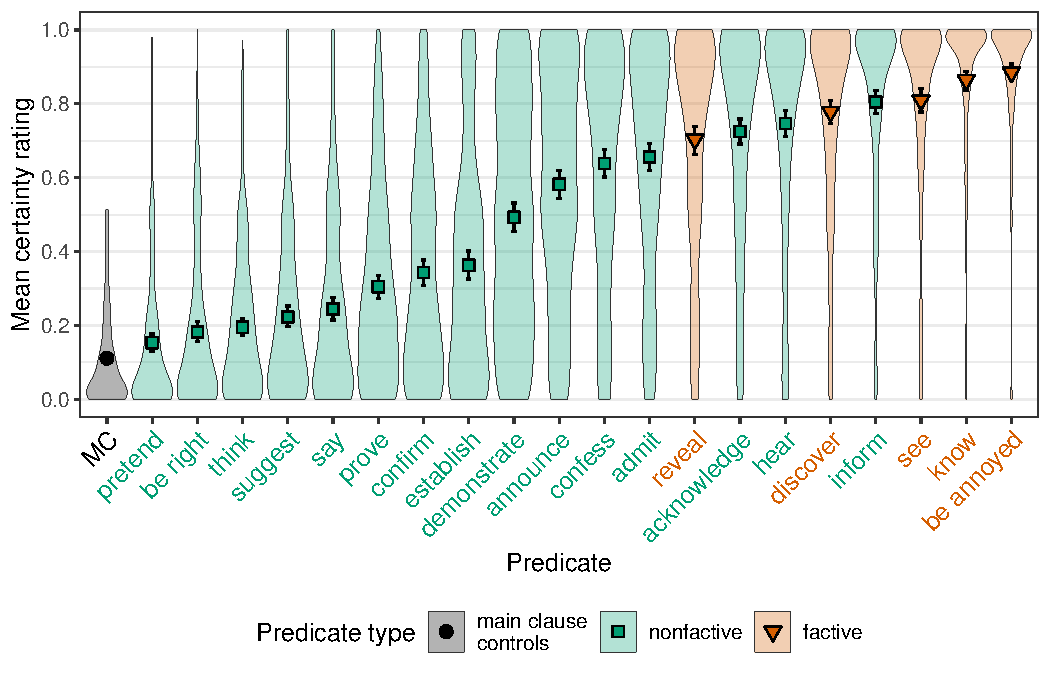
\includegraphics[width=.8\textwidth]{../../results/main/graphs/mean-certainty-by-predicateType}
\caption{Mean certainty rating (measuring projection) of main clause (`MC') content and the CCs of the 20 \color{orange}factive \color{black} and \color{green}nonfactive \color{black} predicates investigated in Exp.~1a of \citealt{degen-tonhauser-language} (adapted by collapsing the nonfactive predicates into a single category). Error bars indicate 95\% bootstrapped confidence intervals. Violin plots indicate the kernel probability density of the individual participants' ratings.}\label{fig:dt1a}
\end{figure}

Recently,  \citealt*[\S6.2]{mandelkern-etal2020} challenged the hypothesis that projection is gradient by arguing that inference rating measures are not suitable to detect categorical projection. Such measures are not suitable, they argued, because they do not distinguish between, on the one hand, contents that project because they are presuppositions and, on the other hand, contents that project because they are ``a natural conclusion to draw for any of a variety of pragmatic reasons short of entailment or presupposition'' (p.497). Inference rating measures, they suggested, might invite participants to draw projection inferences even when not lexically required because ``the content in question is right there before the [participants'] eyes" (p.498). They concluded that ``we should think twice before embracing a notion of presupposition projection that is gradient based on results from inference tasks alone'' (p.497).

\citealt[\S6.2]{mandelkern-etal2020} suggested that naturalness ratings of utterances in explicit ignorance contexts are better suited to distinguish presuppositions from nonpresuppositional projection inferences.\footnote{\citealt{mandelkern-etal2020} refer to the measure as an acceptability rating measure, but since participants were asked to rate the naturalness of utterances, we refer to it as a naturalness rating measure.} On this measure, participants are presented with utterances in which a speaker states that they are ignorant about a content, as in (\ref{mtrig}a), and then follows up with an utterance in which the content occurs embedded in an entailment-canceling environment, such as the antecedent of a conditional in (\ref{mtrig}c). \citealt{mandelkern-etal2020} assumed that if the content is a presupposition (such as the pre-state content of {\em stop} in (\ref{mtrig}c)), the utterance is rated as unnatural in the explicit ignorance context because presuppositions are contents that the speaker believes to be true. That is, in such constellations,  participants ``will not have an alternative to interpreting the presupposition at the utterance level, and in turn seeing the utterance as infelicitous and the speaker as incoherent'' (p.497).  If, on the other hand, the content is not a presupposition (such as the pre-state content of {\em now frown on} in (\ref{mtrig}c)), the utterance is assumed to be natural: Even if participants might in some context draw a projection inference ``for any of a variety of pragmatic reasons short of entailment or presupposition, [\ldots] they will tend to relinquish that inclination when there is pragmatic pressure to do so'', as in the explicit ignorance contexts (p.497). Both presupposition triggers and nontriggers were expected to be judged as natural in the support context, which entails the relevant content, illustrated in (\ref{mtrig}b).

\begin{exe}
\ex\label{mtrig} \citealt[490f.]{mandelkern-etal2020}
\begin{xlist}
\ex Explicit ignorance context: \\ Mary always was involved in a lot of sports, but I don't know whether she ever did any yoga.
\ex Support context: \\ Mary always was involved in a lot of sports, and she used to do yoga, too.
\ex Sentence with presupposition / nonpresupposition: \\ If Mary \{has stopped / now frowns on\} doing yoga, then Matthew will interview her for his story.
\end{xlist}
\end{exe}

In \citepos{mandelkern-etal2020} Exp.~3, which used the proposed measure, items like (\ref{mtrig}) were control items. Mandelkern and colleagues found that the naturalness ratings for nontriggers were relatively high in both contexts (with means just below 5 on their 7-point Likert scale, where 1 meant ``completely unnatural'' and 7 meant ``completely natural''). The presupposition triggers, on the other hand, had a lower mean naturalness rating in the explicit ignorance context (around 3) than in the support context (about 5.3). Mandelkern and colleagues took this to ``establish[] the effectiveness of the methodology'' (p.492). They proposed (p.497):

\begin{quote}

[\ldots] comparing contexts which support the inference to contexts in which it has been made clear that the speaker is ignorant about the inference provides a way to distinguish a broad class of natural and invited pragmatic inferences from those that are really encoded as presuppositions, and thus have no choice but to project. [...]  In methodological terms, we strongly recommend at least a two-pronged approach, with careful attention paid to results stemming from the evaluation of acceptabilty [sic] in different contexts.

\end{quote}

However, the empirical evidence in \citealt{mandelkern-etal2020} for their claim that projection is categorical is weak. This is primarily because the goal of their work was not to investigate this claim, but whether presupposition projection in conjunctions is symmetric. It is also weak, however, because the results (shown in Fig.~8 in their Appendix 3) do not appear to support a categorical distinction between the the presupposition triggers and nontriggers investigated, even though there were only four triggers ({\em be aware, be happy, stop, continue}) and four nontriggers ({\em now frown on, enjoy, hope, be sure}).  First, considering just the mean naturalness ratings in the explicit ignorance context, it appears that the ratings for the presuppositions and nonpresuppositions overlap: The ratings for the presuppositions ranged from 1 (for the pre-state of {\em continue}) to about 3.5 (for the CC of {\em be aware}), and the ratings for the nonpresuppositions range from just below 3 (for the CC of {\em hope}) to 4.5 (for the CC of {\em be aware}). It is therefore not clear that naturalness ratings in explicit ignorance contexts provide evidence for a categorical distinction between the four presuppositions and the four nonpresuppositions investigated in \citealt{mandelkern-etal2020}. Second, there is no consistent effect of context: Whereas the difference between the mean naturalness ratings in the explicit ignorance and support context was quite large for the (presuppositional) pre-state of {\em continue}, the difference was much less pronounced for the (presuppositional) CC of {\em be aware}, where it was roughly comparable to that of the (nonpresuppositional) pre-state of {\em frown on}. Thus, it is not clear that comparisons of ratings in support and explicit ignorance contexts provides empirical support for a categorical projection either. 

Another issue with \citepos{mandelkern-etal2020} claim is that there is disagreement in the literature about the naturalness of presuppositions in explicit ignorance contexts. Whereas Mandelkern and colleagues assumed that all presuppositions are unnatural in explicit ignorance contexts (modulo local accommodation), \citealt{simons01} and \citealt{abusch10} assumed that only `hard' (nondefeasible) presuppositions are, but that `soft' (defeasible) ones are natural. For instance,  the examples with {\em stop}, {\em discover}, and {\em win} in (\ref{eic2}) were assumed to be natural in explicit ignorance contexts, and the examples with {\em again}, the {\em it-}cleft and {\em too} in (\ref{eic3}) unnatural.

\begin{exe}
\ex\label{eic2}
\begin{xlist}
\ex I have no idea whether Jane ever smoked, but she hasn't stopped smoking. \hfill (\citealt[443]{simons01})
\ex Context: ``two people [\ldots] know that Henry is searching for Jane, but who don't themselves know where Jane is:'' \\ If Henry discovers that Jane is in New York, there'll be trouble. \hfill (\citealt[434]{simons01})
\ex I have no idea whether John ended up participating in the
Road Race yesterday. But if he won it, then he has more victories than anyone else in history. \hfill (\citealt[39]{abusch10})
\end{xlist}
\ex\label{eic3}
\begin{xlist}
\ex\infelic I don't know if Jane ever rented ``Manhattan'' before, but perhaps she's renting it again. \hfill (\citealt[443]{simons01})

\ex \verymarginal I have no idea whether anyone read that letter. But if it is John
who read it, let's ask him to be discreet about the content. \hfill (\citealt[40]{abusch10})

\ex \verymarginal I have no idea whether John read that proposal. But if Bill read it too, let's ask them to confer and simply give us a yes-no response. \hfill (\citealt[40]{abusch10})
\end{xlist}
\end{exe}

This paper presents the results of an experiment designed to investigate \citepos{mandelkern-etal2020} claim that the measure they proposed provides evidence that projection is categorical and distinguishes presuppositions from nonpresuppositions.\footnote{\label{f:github}The experiment was approved by the ethics review committee of [university name suppressed]. The experiment, materials, data, and analysis scripts can be accessed here:  \url{xxx} {\bf DO THIS AFTER FINALIZING SCRIPTS}}  To allow for comparison with the results of \citealt{degen-tonhauser-language}, the CCs of the same 20 (non)factive clause-embedding predicates (see Fig.~\ref{fig:dt1a}) were investigated. The experiment also included control stimuli with {\em stop, continue, again, too, also}, and an {\em it-}cleft to allow for comparison with the results of \citealt{mandelkern-etal2020} and the assumptions made in \citealt{simons01} and \citealt{abusch10}. 

The design of \citepos{mandelkern-etal2020} Exp.~3 was slightly modified to allow for comparison with the result of \citealt{degen-tonhauser-openmind} that the projection of content is sensitive to the content's prior probability. Specifically, what \citealt{degen-tonhauser-openmind} found was that the higher the prior probability of a content, the stronger the projection inference. For instance, a speaker's commitment to the CC of (\ref{prior}c), that Julian dances salsa, was stronger in the context in (\ref{prior}b), where the CC has a higher prior probability, than in the context in (\ref{prior}a), where the CC has a lower prior probability.

\begin{exe}
\ex\label{prior}
\begin{xlist}
\ex Julian is German. \hfill [lower prior probability]
\ex Julian is Cuban. \hfill [higher prior probability]
\ex Did Cole discover that Julian dances salsa?
\end{xlist}
\end{exe}
Our experiment replaced \citepos{mandelkern-etal2020} support context that entailed the relevant context with two support contexts that differed in the prior probability of the CC, namely a lower and a higher prior probability context.\footnote{Another change was that participants gave their naturalness ratings on a slider with endpoints labeled `totally unnatural' and `totally natural' rather than on a 7-point Likert scale with endpoints labeled `completely unnatural' and `completely natural'.}  Under analyses of presuppositions like \citealt{heim83} or \citealt{vds92}, presuppositions are by default globally accommodated in contexts that are compatible with the presupposition, like these lower and higher prior probability contexts. Accordingly, such analyses predict that presuppositions are rated as natural in lower and higher probability contexts, just as in \citepos{mandelkern-etal2020} entailing support context. 


\section{Experiment}\label{s2}

To investigate \citepos{mandelkern-etal2020} claim that their naturalness rating measure provides evidence for categorical projection, participants read two-sentence discourses consisting of a declarative (which provided the context) and an interrogative (which realized a factive or nonfactive predicate), and rated the naturalness of the interrogative in the context of the declarative.

\subsection{Methods}\label{s-methods}

\subsubsection{Participants}

We recruited 425 participants on Prolific. Due to a programming error, the data of only 398 participants was recorded (ages: 19-73, mean: 40.8; 187 women, 201 men, 8 non-categorical, 2 preferred to not disclose). The recruited participants were required to live in the USA, to speak English as their first language, to have completed at least 100 tasks, and to have an approval rating of at least 99\%. The median time spent on the task was 6:24 minutes. Participants were paid \$1.78, corresponding to an hourly pay of \$16.6.


\subsubsection{Materials}

Participants read two-sentence discourses consisting of a declarative followed by an interrogative, as shown in (\ref{sample}). In the target stimuli, the interrogatives combined the 20 (non)factive predicates of \citealt{degen-tonhauser-language} (see Fig.~\ref{fig:dt1a}) with the 20 complement clauses of \citealt{degen-tonhauser-language}, for a total of 400 interrogatives. The preceding declaratives implemented a three-level context condition: In the `explicit ignorance' context (\ref{sample}a), the declarative sentence conveyed the speaker's ignorance about the CC. In the `lower prior probability' context (\ref{sample}b), the CC had a comparatively lower prior probability, whereas it had a comparatively higher prior probability in the `higher prior probability' context (\ref{sample}c). The two contexts for each of the 20 complement clauses were normed in \citealt{degen-tonhauser-openmind}. See Supplement \ref{a:clauses} for the full set of 20 complement clauses and the two contexts for each complement clause.

\begin{exe}
\ex\label{sample}
\begin{xlist}
\ex Explicit ignorance context: \\ I have no idea if Julian dances salsa. Does Cole discover that Julian dances salsa?
\ex Lower prior probability context: \\ Julian is German. Did Cole discover that Julian dances salsa?
\ex Higher prior probability context: \\ Julian is Cuban. Did Cole discover that Julian dances salsa?'
\end{xlist}
\end{exe}

In addition to the 1,200 target stimuli (400 interrogatives $\times$ 3 contexts), the materials also included the six control stimuli in (\ref{filler}). The interrogatives of the control stimuli featured six expressions typically analyzed as presupposition triggers, namely {\em stop, continue, again, too, also}, and an {\em it-}cleft. The preceding declaratives conveyed the speaker's explicit ignorance about the presuppositions associated with these expressions.\footnote{The contents investigated for {\em too} and {\em also} in (\ref{filler}d) and (\ref{filler}e) are that Ann plays an instrument other than the flute and that Svenja plays a sport other than soccer. This interpretation arises if {\em too} and {\em also} associate with {\em the flute} and {\em soccer}, respectively. While prosody was not controlled for, this focus association is made plausible by the preceding explicit ignorance statements, which evoke the question of whether Ann plays any instrument and whether Svenja plays any sport, respectively.} Two of these expressions, namely {\em stop} and {\em continue}, were target expressions in \citepos{mandelkern-etal2020} Exp.~3, where they were assumed to be unnatural in explicit ignorance contexts. This is in contrast to \citealt{simons01}, who took {\em stop} to be a soft trigger that is natural in explicit ignorance contexts. Three expressions were assumed to be unnatural in explicit ignorance contexts in \citealt{simons01} ({\em again}) and \citealt{abusch10} ({\em too}, {\em it-}cleft). The control stimuli were included for comparison to the target stimuli, to the claims of \citealt{simons01} and \citealt{abusch10}, and to the results of \citealt{mandelkern-etal2020}.

\begin{exe}
\ex\label{filler} 
\begin{xlist}
\ex I don't know if Stephen was ever in the habit of vaping. Has Stephen recently stopped vaping?
\ex I don't know if John was ever reading ``Dune''. Has John recently continued reading ``Dune''?
\ex I don't know if William was ever interested in history. Is William interested in history again?"
\ex I don't know if Ann plays any instrument. Does Ann play the flute, too?
\ex I don't know if Svenja plays any sport. Does Svenja also play soccer?
\ex I don't know if anyone was playing outside with the kids. Was it Jack who was playing outside with the kids?

\end{xlist}
\end{exe}

The experiment also included 4 filler stimuli that were used to exclude participants not attending to the task (see Supplement \ref{a:fillerPractice}). The filler stimuli were expected to receive high naturalness ratings.

A random set of 30 stimuli was created for each participant. Each set contained 20 target stimuli in which each of the 20 complement clauses was paired with a unique clause-embedding predicate. Twelve of the target stimuli were presented in the explicit ignorance context, and the other eight in a low or a higher prior probability context (four each). Each participants' set also contained the same six control stimuli and the same four filler stimuli. Each of the 30 stimuli were presented as utterances by a unique named speaker. Trial order was randomized for each participant. 

\subsubsection{Procedure}

Participants were instructed to rate how natural the question sounds in the context of the statement. As shown in Figure \ref{f:trials}, they were asked give their rating on a slider from `totally unnatural' (coded as 0) to `totally natural' (coded as 1). The experiment began with four practice trials to familiarize participants with the task (see Supplement \ref{a:fillerPractice} for details). After rating the 30 trials, participants filled out a short optional demographic survey. To encourage truthful responses, participants were told that they would be paid no matter what answers they gave in the survey.


\begin{figure}[h]
\centering
%\begin{subfigure}{0.49\textwidth}
\fbox{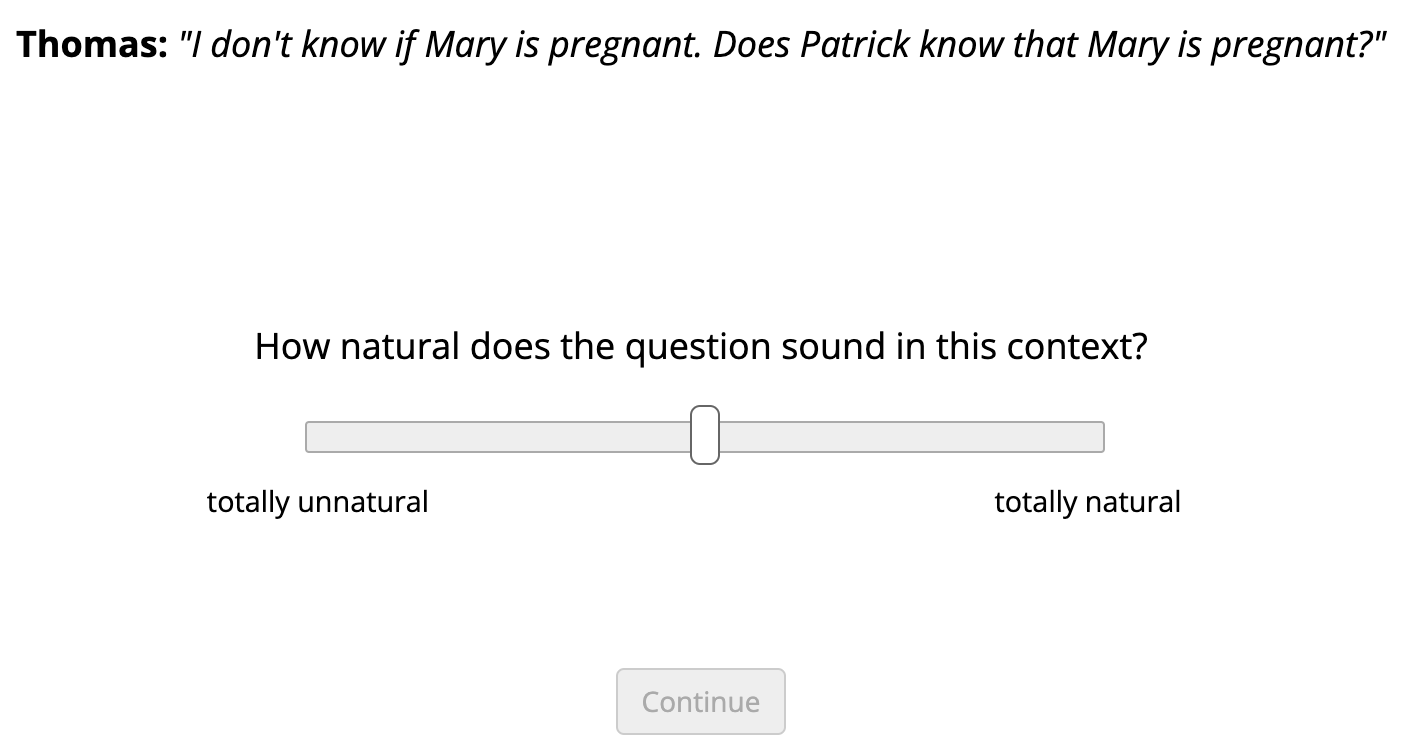
\includegraphics[width=.7\textwidth]{figures/trial-eic}}
%\caption{Trial with explicit ignorance context}
%\end{subfigure}
%\\[.1cm]
%\begin{subfigure}{0.49\textwidth}
%\fbox{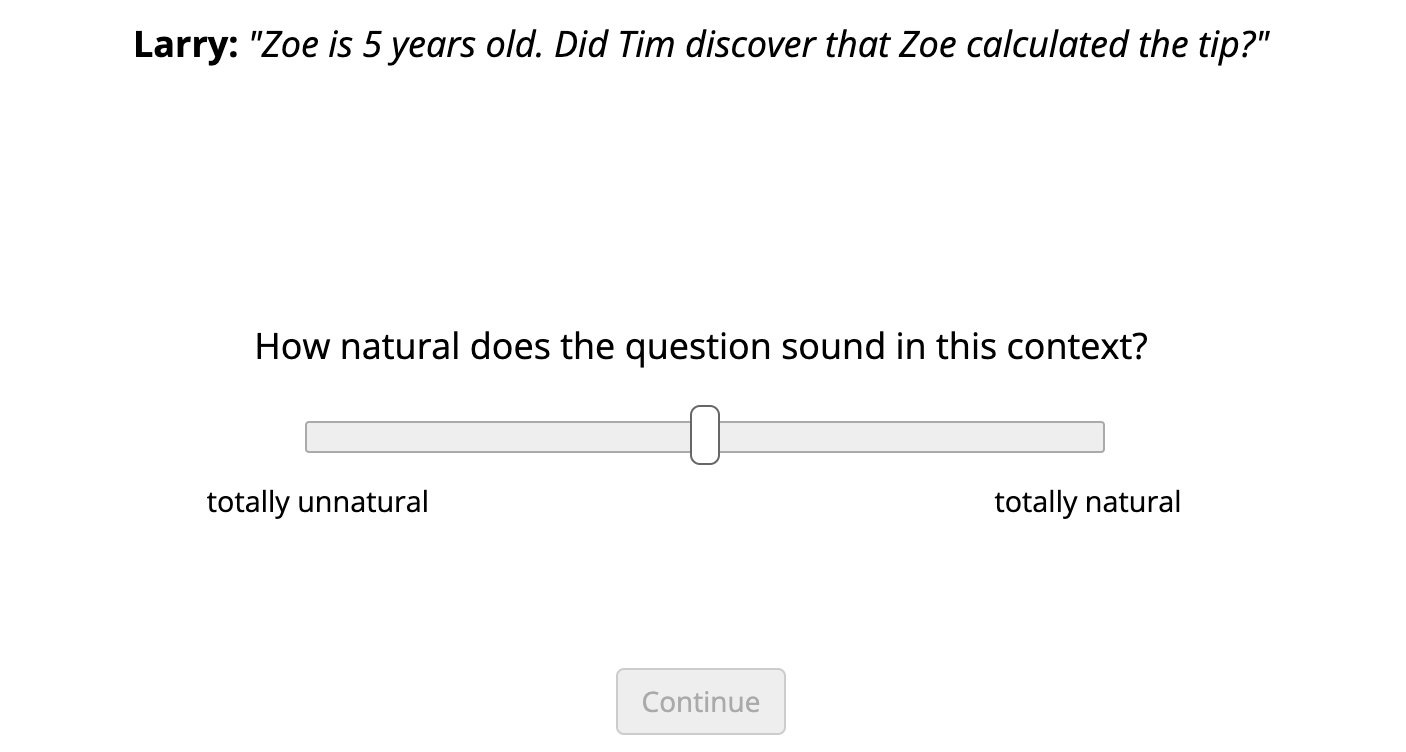
\includegraphics[width=\textwidth]{figures/trial-low}}
%\caption{Trial with lower prior probability context}
%\end{subfigure} \hfill \begin{subfigure}{0.49\textwidth}
%\fbox{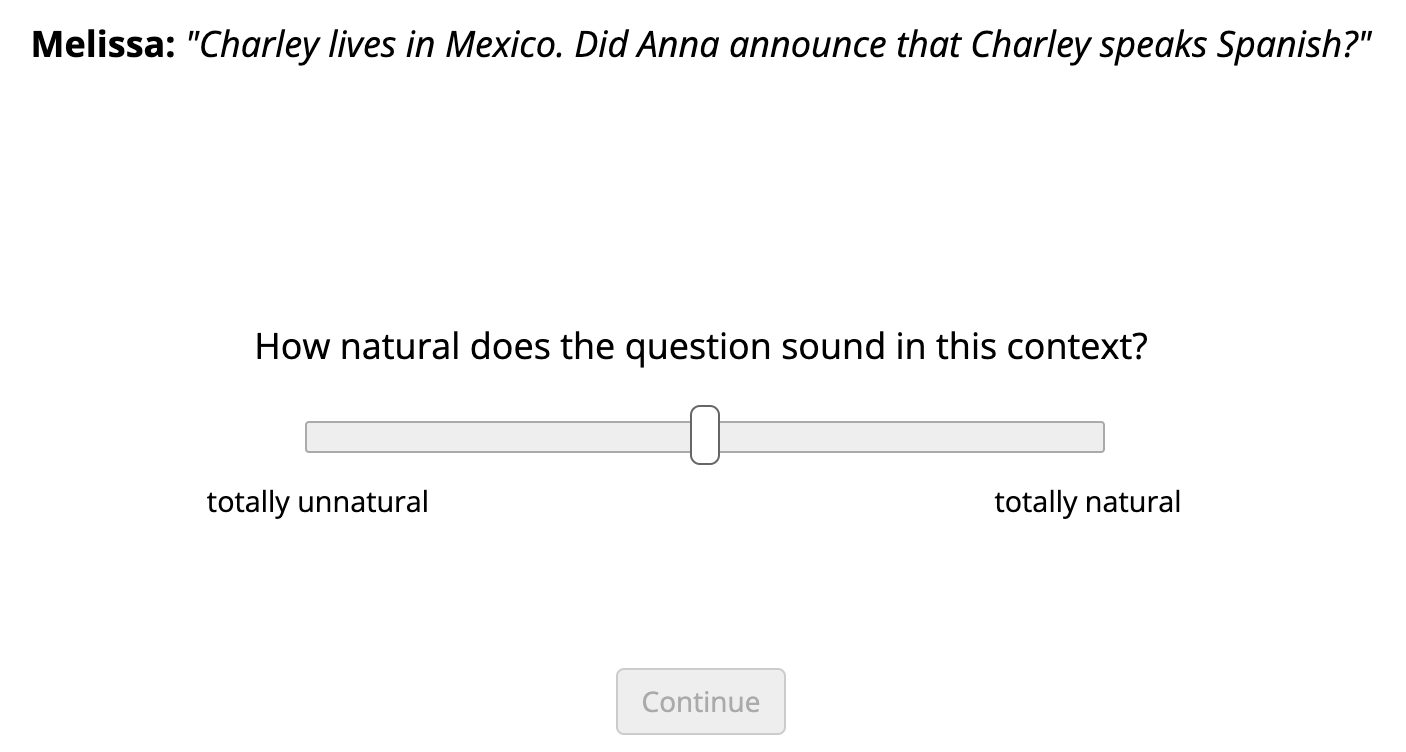
\includegraphics[width=\textwidth]{figures/trial-high}}
%\caption{Trial with higher prior probability context}
%\end{subfigure}
\caption{Sample trial with explicit ignorance context.}\label{f:trials}
\end{figure}


\subsubsection{Data exclusion} 

We excluded the data of 5 participants who did not self-identify as native speakers of American English and that of 23 participants whose mean response to the fillers (expected to be natural) was more than 2 sd below the group mean.\footnote{Contrary to what was planned, one of the four filler stimuli was not used to exclude participants' data because it received a mean rating of only .5. See Supplement \ref{a:fillerPractice} for details.} The data of 370 participants entered into the analysis (ages: 19-80, mean: 40.7; 175 women, 185 men, 8 nonbinary, 2 did not disclose). The 20 predicates each received at least 200 ratings in the explicit ignorance context (mean: 222 ratings), at least 59 ratings in the lower prior probability context (mean: 74), and at least 61 ratings in the higher prior probability context (mean: 74). The six controls received 370 ratings each. 

\subsection{Results and discussion}

We first address the question of whether naturalness ratings in explicit ignorance contexts provide empirical evidence for categorical projection (\S\ref{s:analysis1}). We then consider whether a comparison of naturalness ratings in the three contexts provides such evidence (\S\ref{s:analysis2}).

\subsubsection{Naturalness ratings in explicit ignorance contexts}\label{s:analysis1}

\paragraph{Results.} Recall that \citealt{simons01} and \citealt{abusch10} assumed that only hard presuppositions are unnatural in explicit ignorance contexts, whereas \citealt{mandelkern-etal2020} assumed that all presuppositions are unnatural in such contexts. Figure \ref{fig:acc-by-expression} shows mean naturalness ratings in the explicit ignorance context by expression (in distinct colors: \color{orange}factive predicates\color{black}, \color{green}nonfactive predicates\color{black},  controls). As shown, the purported presupposition triggers, that is, the controls and the factive predicates, do not exhibit a unified pattern: The means of four controls ({\em continue, too, also, again}) are at floor, those of {\em stop} and {\em be annoyed} are slightly higher, those of the {\em it-}cleft and {\em know} are higher again, but lower than those of {\em see} and {\em discover}, and, finally, those of {\em reveal} are highest. We also see that the naturalness ratings of {\em see, discover} and {\em reveal} are just as high as those of some nonfactive predicates. These results do not provide empirical support for a categorical distinction between presuppositions and nonpresuppositions, contrary to what \citealt{mandelkern-etal2020} claimed. These results also do not provide support for a class of factive predicates that is categorically distinct from nonfactive ones, in line with the result of \citealt{degen-tonhauser-language} based on inference rating measures. 

\begin{figure}[h!]
\centering
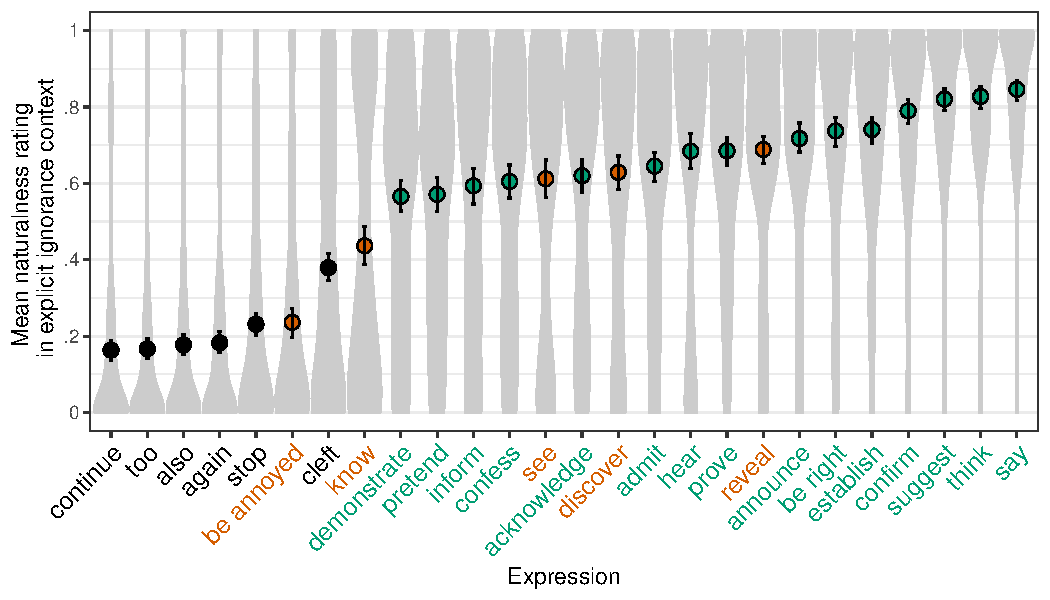
\includegraphics[width=.9\textwidth]{../../results/main/graphs/explicit-ignorance-naturalness-by-predicate}
\caption{Mean naturalness rating in explicit ignorance context by expression (\color{orange}factive\color{black}, \color{green}nonfactive\color{green}, \color{black}filler\color{black}). Error bars indicate 95\% bootstrapped confidence intervals. Overlaid violin plots indicate the kernel probability density of the participants' ratings.}\label{fig:acc-by-expression}
\end{figure}

These observations were confirmed by a posthoc pairwise comparison of the estimated means for each control and target expression in the explicit ignorance context using the `emmeans' package (\citealt{emmeans}) in R (\citealt{r}). The input to the pairwise comparison was a Bayesian mixed-effects beta regression model with weakly informative priors that was fit using the `brms' package (\citealt{buerkner2017}). The model predicted naturalness ratings\footnote{To model the ratings using a beta regression, the ratings were first transformed from the interval [0,1] to the interval (0,1) using the method proposed in \citealt{smithson-verkuilen2006}.} from a fixed effect of expression (with treatment coding and `continue' as reference level) and included random by-participant and by-item intercepts (where an item is a complement clause). The output of the pairwise comparison were 95\% highest density intervals (HDIs) of estimated marginal mean differences between each of the expressions. We assume that two expressions differ in their naturalness in the explicit ignorance context if their HDI does not include 0.

As shown in Table \ref{t:pairwise},\footnote{While the naturalness ratings collected from the participants range from 0 to 1, the greater than $|$1$|$  estimated marginal mean differences are the result of the beta regression using a logit link function for the mean parameter. The full model output is available here: \url{LINK TO TABLE IN REPO} {\bf ADD THIS AFTER FINALIZING SCRIPTS}.} the pairwise comparison suggests differences between the naturalness ratings of the CCs of the five factive predicates: The ratings of {\em be annoyed} are lower than those of {\em know}, which in turn are lower than those of {\em see} and {\em discover}, which in turn are lower than those of {\em reveal}. There is also variation between the factive predicates and the presuppositional controls: While all five factive predicates are more natural in explicit ignorance contexts than {\em continue, too} and {\em also}, {\em know} is additionally more natural than {\em again} and {\em stop}, and {\em see, discover} and {\em reveal} are additionally more natural than the {\em it-}cleft. Finally, the naturalness ratings in explicit ignorance contexts for {\em see} and {\em discover} do not differ from those of the nonfactives {\em confess, inform}, and {\em acknowledge}, and those of {\em reveal} do not differ from those of the nonfactives {\em admit, hear}, and {\em prove}. These results suggest that naturalness ratings in explicit ignorance contexts do not provide empirical support for categorical projection or for a categorical distinction between factive and nonfactive predicates. 

\begin{table}[!h]
\addtolength{\tabcolsep}{-.19em}
\centering
\begin{tabular}{r | cccccccccccccccccccccccccc}
& \rots{\bf continue} & \rots{\bf too} & \rots{\bf also} & \rots{\bf again} & \rots{\bf stop} & \rots{\color{orange}{\bf be annoyed}\color{black}} & \rots{\bf cleft} & \rots{\color{orange}{\bf know}\color{black}} & \rots{\color{green}{\bf demonstrate}\color{black}} & \rots{\color{green}{\bf pretend}\color{black}} & \rots{\color{green}{\bf inform}\color{black}} & \rots{\color{green}{\bf confess}\color{black}} & \rots{\color{orange}{\bf see}\color{black}} & \rots{\color{green}{\bf acknowledge}\color{black}} & \rots{\color{orange}{\bf discover}\color{black}} & \rots{\color{green}{\bf admit}\color{black}} & \rots{\color{green}{\bf hear}\color{black}} & \rots{\color{green}{\bf prove}\color{black}} & \rots{\color{orange}{\bf reveal}\color{black}} & \rots{\color{green}{\bf announce}\color{black}} & \rots{\color{green}{\bf be right}\color{black}} & \rots{\color{green}{\bf establish}\color{black}} & \rots{\color{green}{\bf confirm}\color{black}} & \rots{\color{green}{\bf suggest}\color{black}} & \rots{\color{green}{\bf think}\color{black}} & \rots{\color{green}{\bf say}\color{black}} \\
\hline
 {\bf continue} & \cellcolor{black} & \cellcolor{white} & \cellcolor{white} & \cellcolor{white} & \cellcolor{yellow3} & \cellcolor{yellow3} & \cellcolor{yellow2} & \cellcolor{yellow2} & \cellcolor{yellow1} & \cellcolor{yellow1} & \cellcolor{yellow1} & \cellcolor{yellow1} & \cellcolor{yellow1} & \cellcolor{yellow1} & \cellcolor{yellow1} & \cellcolor{yellow1} & \cellcolor{yellow1} & \cellcolor{yellow1} & \cellcolor{yellow1} & \cellcolor{yellow1} & \cellcolor{yellow1} & \cellcolor{yellow1} & \cellcolor{yellow1} & \cellcolor{yellow1} & \cellcolor{yellow1} & \cellcolor{yellow1} \\ 
  {\bf too} & \cellcolor{white} & \cellcolor{black} & \cellcolor{white} & \cellcolor{white} & \cellcolor{yellow3} & \cellcolor{yellow3} & \cellcolor{yellow2} & \cellcolor{yellow2} & \cellcolor{yellow1} & \cellcolor{yellow1} & \cellcolor{yellow1} & \cellcolor{yellow1} & \cellcolor{yellow1} & \cellcolor{yellow1} & \cellcolor{yellow1} & \cellcolor{yellow1} & \cellcolor{yellow1} & \cellcolor{yellow1} & \cellcolor{yellow1} & \cellcolor{yellow1} & \cellcolor{yellow1} & \cellcolor{yellow1} & \cellcolor{yellow1} & \cellcolor{yellow1} & \cellcolor{yellow1} & \cellcolor{yellow1} \\ 
  {\bf also} & \cellcolor{white} & \cellcolor{white} & \cellcolor{black} & \cellcolor{white} & \cellcolor{yellow3} & \cellcolor{yellow3} & \cellcolor{yellow2} & \cellcolor{yellow2} & \cellcolor{yellow2} & \cellcolor{yellow1} & \cellcolor{yellow1} & \cellcolor{yellow1} & \cellcolor{yellow1} & \cellcolor{yellow1} & \cellcolor{yellow1} & \cellcolor{yellow1} & \cellcolor{yellow1} & \cellcolor{yellow1} & \cellcolor{yellow1} & \cellcolor{yellow1} & \cellcolor{yellow1} & \cellcolor{yellow1} & \cellcolor{yellow1} & \cellcolor{yellow1} & \cellcolor{yellow1} & \cellcolor{yellow1} \\ 
  {\bf again} & \cellcolor{white} & \cellcolor{white} & \cellcolor{white} & \cellcolor{black} & \cellcolor{yellow3} & \cellcolor{white} & \cellcolor{yellow2} & \cellcolor{yellow2} & \cellcolor{yellow2} & \cellcolor{yellow2} & \cellcolor{yellow2} & \cellcolor{yellow1} & \cellcolor{yellow1} & \cellcolor{yellow1} & \cellcolor{yellow1} & \cellcolor{yellow1} & \cellcolor{yellow1} & \cellcolor{yellow1} & \cellcolor{yellow1} & \cellcolor{yellow1} & \cellcolor{yellow1} & \cellcolor{yellow1} & \cellcolor{yellow1} & \cellcolor{yellow1} & \cellcolor{yellow1} & \cellcolor{yellow1} \\ 
  {\bf stop} & \cellcolor{purple3} & \cellcolor{purple3} & \cellcolor{purple3} & \cellcolor{purple3} & \cellcolor{black} & \cellcolor{white} & \cellcolor{yellow2} & \cellcolor{yellow2} & \cellcolor{yellow2} & \cellcolor{yellow2} & \cellcolor{yellow2} & \cellcolor{yellow2} & \cellcolor{yellow2} & \cellcolor{yellow2} & \cellcolor{yellow2} & \cellcolor{yellow2} & \cellcolor{yellow1} & \cellcolor{yellow1} & \cellcolor{yellow1} & \cellcolor{yellow1} & \cellcolor{yellow1} & \cellcolor{yellow1} & \cellcolor{yellow1} & \cellcolor{yellow1} & \cellcolor{yellow1} & \cellcolor{yellow1} \\ 
  \color{orange}{\bf be annoyed}\color{black} & \cellcolor{purple3} & \cellcolor{purple3} & \cellcolor{purple3} & \cellcolor{white} & \cellcolor{white} & \cellcolor{black} & \cellcolor{yellow2} & \cellcolor{yellow2} & \cellcolor{yellow2} & \cellcolor{yellow2} & \cellcolor{yellow2} & \cellcolor{yellow2} & \cellcolor{yellow2} & \cellcolor{yellow2} & \cellcolor{yellow2} & \cellcolor{yellow2} & \cellcolor{yellow1} & \cellcolor{yellow1} & \cellcolor{yellow1} & \cellcolor{yellow1} & \cellcolor{yellow1} & \cellcolor{yellow1} & \cellcolor{yellow1} & \cellcolor{yellow1} & \cellcolor{yellow1} & \cellcolor{yellow1} \\ 
  {\bf cleft} & \cellcolor{purple2} & \cellcolor{purple2} & \cellcolor{purple2} & \cellcolor{purple2} & \cellcolor{purple2} & \cellcolor{purple2} & \cellcolor{black} & \cellcolor{white} & \cellcolor{yellow2} & \cellcolor{yellow2} & \cellcolor{yellow2} & \cellcolor{yellow2} & \cellcolor{yellow2} & \cellcolor{yellow2} & \cellcolor{yellow2} & \cellcolor{yellow2} & \cellcolor{yellow2} & \cellcolor{yellow2} & \cellcolor{yellow2} & \cellcolor{yellow2} & \cellcolor{yellow2} & \cellcolor{yellow2} & \cellcolor{yellow1} & \cellcolor{yellow1} & \cellcolor{yellow1} & \cellcolor{yellow1} \\ 
  \color{orange}{\bf know}\color{black} & \cellcolor{purple2} & \cellcolor{purple2} & \cellcolor{purple2} & \cellcolor{purple2} & \cellcolor{purple2} & \cellcolor{purple2} & \cellcolor{white} & \cellcolor{black} & \cellcolor{yellow3} & \cellcolor{yellow3} & \cellcolor{yellow2} & \cellcolor{yellow2} & \cellcolor{yellow2} & \cellcolor{yellow2} & \cellcolor{yellow2} & \cellcolor{yellow2} & \cellcolor{yellow2} & \cellcolor{yellow2} & \cellcolor{yellow2} & \cellcolor{yellow2} & \cellcolor{yellow2} & \cellcolor{yellow2} & \cellcolor{yellow2} & \cellcolor{yellow2} & \cellcolor{yellow1} & \cellcolor{yellow1} \\ 
  \color{green}{\bf demonstrate}\color{black} & \cellcolor{purple1} & \cellcolor{purple1} & \cellcolor{purple2} & \cellcolor{purple2} & \cellcolor{purple2} & \cellcolor{purple2} & \cellcolor{purple2} & \cellcolor{purple3} & \cellcolor{black} & \cellcolor{white} & \cellcolor{white} & \cellcolor{yellow3} & \cellcolor{yellow3} & \cellcolor{white} & \cellcolor{white} & \cellcolor{yellow3} & \cellcolor{yellow3} & \cellcolor{yellow3} & \cellcolor{yellow3} & \cellcolor{yellow2} & \cellcolor{yellow2} & \cellcolor{yellow2} & \cellcolor{yellow2} & \cellcolor{yellow2} & \cellcolor{yellow2} & \cellcolor{yellow2} \\ 
  \color{green}{\bf pretend}\color{black} & \cellcolor{purple1} & \cellcolor{purple1} & \cellcolor{purple1} & \cellcolor{purple2} & \cellcolor{purple2} & \cellcolor{purple2} & \cellcolor{purple2} & \cellcolor{purple3} & \cellcolor{white} & \cellcolor{black} & \cellcolor{white} & \cellcolor{white} & \cellcolor{white} & \cellcolor{white} & \cellcolor{white} & \cellcolor{yellow3} & \cellcolor{yellow3} & \cellcolor{yellow3} & \cellcolor{yellow3} & \cellcolor{yellow2} & \cellcolor{yellow2} & \cellcolor{yellow2} & \cellcolor{yellow2} & \cellcolor{yellow2} & \cellcolor{yellow2} & \cellcolor{yellow2} \\ 
  \color{green}{\bf inform}\color{black} & \cellcolor{purple1} & \cellcolor{purple1} & \cellcolor{purple1} & \cellcolor{purple2} & \cellcolor{purple2} & \cellcolor{purple2} & \cellcolor{purple2} & \cellcolor{purple2} & \cellcolor{white} & \cellcolor{white} & \cellcolor{black} & \cellcolor{white} & \cellcolor{white} & \cellcolor{white} & \cellcolor{white} & \cellcolor{yellow3} & \cellcolor{yellow3} & \cellcolor{yellow3} & \cellcolor{yellow3} & \cellcolor{yellow2} & \cellcolor{yellow3} & \cellcolor{yellow2} & \cellcolor{yellow2} & \cellcolor{yellow2} & \cellcolor{yellow2} & \cellcolor{yellow2} \\ 
  \color{green}{\bf confess}\color{black} & \cellcolor{purple1} & \cellcolor{purple1} & \cellcolor{purple1} & \cellcolor{purple1} & \cellcolor{purple2} & \cellcolor{purple2} & \cellcolor{purple2} & \cellcolor{purple2} & \cellcolor{purple3} & \cellcolor{white} & \cellcolor{white} & \cellcolor{black} & \cellcolor{white} & \cellcolor{white} & \cellcolor{white} & \cellcolor{white} & \cellcolor{yellow3} & \cellcolor{white} & \cellcolor{white} & \cellcolor{yellow3} & \cellcolor{yellow3} & \cellcolor{yellow3} & \cellcolor{yellow2} & \cellcolor{yellow2} & \cellcolor{yellow2} & \cellcolor{yellow2} \\ 
  \color{orange}{\bf see}\color{black} & \cellcolor{purple1} & \cellcolor{purple1} & \cellcolor{purple1} & \cellcolor{purple1} & \cellcolor{purple2} & \cellcolor{purple2} & \cellcolor{purple2} & \cellcolor{purple2} & \cellcolor{purple3} & \cellcolor{white} & \cellcolor{white} & \cellcolor{white} & \cellcolor{black} & \cellcolor{white} & \cellcolor{white} & \cellcolor{white} & \cellcolor{yellow3} & \cellcolor{white} & \cellcolor{yellow3} & \cellcolor{yellow3} & \cellcolor{yellow3} & \cellcolor{yellow3} & \cellcolor{yellow2} & \cellcolor{yellow2} & \cellcolor{yellow2} & \cellcolor{yellow2} \\ 
  \color{green}{\bf acknowledge}\color{black} & \cellcolor{purple1} & \cellcolor{purple1} & \cellcolor{purple1} & \cellcolor{purple1} & \cellcolor{purple2} & \cellcolor{purple2} & \cellcolor{purple2} & \cellcolor{purple2} & \cellcolor{white} & \cellcolor{white} & \cellcolor{white} & \cellcolor{white} & \cellcolor{white} & \cellcolor{black} & \cellcolor{white} & \cellcolor{white} & \cellcolor{yellow3} & \cellcolor{yellow3} & \cellcolor{yellow3} & \cellcolor{yellow3} & \cellcolor{yellow3} & \cellcolor{yellow2} & \cellcolor{yellow2} & \cellcolor{yellow2} & \cellcolor{yellow2} & \cellcolor{yellow2} \\ 
  \color{orange}{\bf discover}\color{black} & \cellcolor{purple1} & \cellcolor{purple1} & \cellcolor{purple1} & \cellcolor{purple1} & \cellcolor{purple2} & \cellcolor{purple2} & \cellcolor{purple2} & \cellcolor{purple2} & \cellcolor{white} & \cellcolor{white} & \cellcolor{white} & \cellcolor{white} & \cellcolor{white} & \cellcolor{white} & \cellcolor{black} & \cellcolor{white} & \cellcolor{yellow3} & \cellcolor{yellow3} & \cellcolor{yellow3} & \cellcolor{yellow3} & \cellcolor{yellow3} & \cellcolor{yellow2} & \cellcolor{yellow2} & \cellcolor{yellow2} & \cellcolor{yellow2} & \cellcolor{yellow2} \\ 
  \color{green}{\bf admit}\color{black} & \cellcolor{purple1} & \cellcolor{purple1} & \cellcolor{purple1} & \cellcolor{purple1} & \cellcolor{purple2} & \cellcolor{purple2} & \cellcolor{purple2} & \cellcolor{purple2} & \cellcolor{purple3} & \cellcolor{purple3} & \cellcolor{purple3} & \cellcolor{white} & \cellcolor{white} & \cellcolor{white} & \cellcolor{white} & \cellcolor{black} & \cellcolor{white} & \cellcolor{white} & \cellcolor{white} & \cellcolor{yellow3} & \cellcolor{yellow3} & \cellcolor{yellow3} & \cellcolor{yellow2} & \cellcolor{yellow2} & \cellcolor{yellow2} & \cellcolor{yellow2} \\ 
  \color{green}{\bf hear}\color{black} & \cellcolor{purple1} & \cellcolor{purple1} & \cellcolor{purple1} & \cellcolor{purple1} & \cellcolor{purple1} & \cellcolor{purple1} & \cellcolor{purple2} & \cellcolor{purple2} & \cellcolor{purple3} & \cellcolor{purple3} & \cellcolor{purple3} & \cellcolor{purple3} & \cellcolor{purple3} & \cellcolor{purple3} & \cellcolor{purple3} & \cellcolor{white} & \cellcolor{black} & \cellcolor{white} & \cellcolor{white} & \cellcolor{white} & \cellcolor{white} & \cellcolor{yellow3} & \cellcolor{yellow3} & \cellcolor{yellow2} & \cellcolor{yellow2} & \cellcolor{yellow2} \\ 
  \color{green}{\bf prove}\color{black} & \cellcolor{purple1} & \cellcolor{purple1} & \cellcolor{purple1} & \cellcolor{purple1} & \cellcolor{purple1} & \cellcolor{purple1} & \cellcolor{purple2} & \cellcolor{purple2} & \cellcolor{purple3} & \cellcolor{purple3} & \cellcolor{purple3} & \cellcolor{white} & \cellcolor{white} & \cellcolor{purple3} & \cellcolor{purple3} & \cellcolor{white} & \cellcolor{white} & \cellcolor{black} & \cellcolor{white} & \cellcolor{yellow3} & \cellcolor{yellow3} & \cellcolor{yellow3} & \cellcolor{yellow2} & \cellcolor{yellow2} & \cellcolor{yellow2} & \cellcolor{yellow2} \\ 
  \color{orange}{\bf reveal}\color{black} & \cellcolor{purple1} & \cellcolor{purple1} & \cellcolor{purple1} & \cellcolor{purple1} & \cellcolor{purple1} & \cellcolor{purple1} & \cellcolor{purple2} & \cellcolor{purple2} & \cellcolor{purple3} & \cellcolor{purple3} & \cellcolor{purple3} & \cellcolor{white} & \cellcolor{purple3} & \cellcolor{purple3} & \cellcolor{purple3} & \cellcolor{white} & \cellcolor{white} & \cellcolor{white} & \cellcolor{black} & \cellcolor{yellow3} & \cellcolor{white} & \cellcolor{yellow3} & \cellcolor{yellow2} & \cellcolor{yellow2} & \cellcolor{yellow2} & \cellcolor{yellow2} \\ 
  \color{green}{\bf announce}\color{black} & \cellcolor{purple1} & \cellcolor{purple1} & \cellcolor{purple1} & \cellcolor{purple1} & \cellcolor{purple1} & \cellcolor{purple1} & \cellcolor{purple2} & \cellcolor{purple2} & \cellcolor{purple2} & \cellcolor{purple2} & \cellcolor{purple2} & \cellcolor{purple3} & \cellcolor{purple3} & \cellcolor{purple3} & \cellcolor{purple3} & \cellcolor{purple3} & \cellcolor{white} & \cellcolor{purple3} & \cellcolor{purple3} & \cellcolor{black} & \cellcolor{white} & \cellcolor{white} & \cellcolor{yellow3} & \cellcolor{yellow3} & \cellcolor{yellow3} & \cellcolor{yellow2} \\ 
  \color{green}{\bf be right}\color{black} & \cellcolor{purple1} & \cellcolor{purple1} & \cellcolor{purple1} & \cellcolor{purple1} & \cellcolor{purple1} & \cellcolor{purple1} & \cellcolor{purple2} & \cellcolor{purple2} & \cellcolor{purple2} & \cellcolor{purple2} & \cellcolor{purple3} & \cellcolor{purple3} & \cellcolor{purple3} & \cellcolor{purple3} & \cellcolor{purple3} & \cellcolor{purple3} & \cellcolor{white} & \cellcolor{purple3} & \cellcolor{white} & \cellcolor{white} & \cellcolor{black} & \cellcolor{white} & \cellcolor{yellow3} & \cellcolor{yellow3} & \cellcolor{yellow2} & \cellcolor{yellow2} \\ 
  \color{green}{\bf establish}\color{black} & \cellcolor{purple1} & \cellcolor{purple1} & \cellcolor{purple1} & \cellcolor{purple1} & \cellcolor{purple1} & \cellcolor{purple1} & \cellcolor{purple2} & \cellcolor{purple2} & \cellcolor{purple2} & \cellcolor{purple2} & \cellcolor{purple2} & \cellcolor{purple3} & \cellcolor{purple3} & \cellcolor{purple2} & \cellcolor{purple2} & \cellcolor{purple3} & \cellcolor{purple3} & \cellcolor{purple3} & \cellcolor{purple3} & \cellcolor{white} & \cellcolor{white} & \cellcolor{black} & \cellcolor{yellow3} & \cellcolor{yellow3} & \cellcolor{yellow3} & \cellcolor{yellow2} \\ 
  \color{green}{\bf confirm}\color{black} & \cellcolor{purple1} & \cellcolor{purple1} & \cellcolor{purple1} & \cellcolor{purple1} & \cellcolor{purple1} & \cellcolor{purple1} & \cellcolor{purple1} & \cellcolor{purple2} & \cellcolor{purple2} & \cellcolor{purple2} & \cellcolor{purple2} & \cellcolor{purple2} & \cellcolor{purple2} & \cellcolor{purple2} & \cellcolor{purple2} & \cellcolor{purple2} & \cellcolor{purple3} & \cellcolor{purple2} & \cellcolor{purple2} & \cellcolor{purple3} & \cellcolor{purple3} & \cellcolor{purple3} & \cellcolor{black} & \cellcolor{white} & \cellcolor{white} & \cellcolor{yellow3} \\ 
  \color{green}{\bf suggest}\color{black} & \cellcolor{purple1} & \cellcolor{purple1} & \cellcolor{purple1} & \cellcolor{purple1} & \cellcolor{purple1} & \cellcolor{purple1} & \cellcolor{purple1} & \cellcolor{purple2} & \cellcolor{purple2} & \cellcolor{purple2} & \cellcolor{purple2} & \cellcolor{purple2} & \cellcolor{purple2} & \cellcolor{purple2} & \cellcolor{purple2} & \cellcolor{purple2} & \cellcolor{purple2} & \cellcolor{purple2} & \cellcolor{purple2} & \cellcolor{purple3} & \cellcolor{purple3} & \cellcolor{purple3} & \cellcolor{white} & \cellcolor{black} & \cellcolor{white} & \cellcolor{white} \\ 
  \color{green}{\bf think}\color{black} & \cellcolor{purple1} & \cellcolor{purple1} & \cellcolor{purple1} & \cellcolor{purple1} & \cellcolor{purple1} & \cellcolor{purple1} & \cellcolor{purple1} & \cellcolor{purple1} & \cellcolor{purple2} & \cellcolor{purple2} & \cellcolor{purple2} & \cellcolor{purple2} & \cellcolor{purple2} & \cellcolor{purple2} & \cellcolor{purple2} & \cellcolor{purple2} & \cellcolor{purple2} & \cellcolor{purple2} & \cellcolor{purple2} & \cellcolor{purple3} & \cellcolor{purple2} & \cellcolor{purple3} & \cellcolor{white} & \cellcolor{white} & \cellcolor{black} & \cellcolor{white} \\ 
  \color{green}{\bf say}\color{black} & \cellcolor{purple1} & \cellcolor{purple1} & \cellcolor{purple1} & \cellcolor{purple1} & \cellcolor{purple1} & \cellcolor{purple1} & \cellcolor{purple1} & \cellcolor{purple1} & \cellcolor{purple2} & \cellcolor{purple2} & \cellcolor{purple2} & \cellcolor{purple2} & \cellcolor{purple2} & \cellcolor{purple2} & \cellcolor{purple2} & \cellcolor{purple2} & \cellcolor{purple2} & \cellcolor{purple2} & \cellcolor{purple2} & \cellcolor{purple2} & \cellcolor{purple2} & \cellcolor{purple2} & \cellcolor{purple3} & \cellcolor{white} & \cellcolor{white} & \cellcolor{black} \\ 
  

\hline
\end{tabular}
\caption{Pairwise differences between expressions in the explicit ignorance context. The color coding indicates whether the difference between the means of row expressions and column expressions was positive or negative, as well as the size of the difference. A white cell means that the 95\% HDI included 0.\\
Positive difference: \colorbox{purple1}{\makebox[4em][c]{$>=1.5$}}, \colorbox{purple2}{\makebox[4em][c]{($1.5,0.5]$}}, 
\colorbox{purple3}{\makebox[4em][c]{($0.5, 0]$}} \\
Negative difference: \colorbox{yellow1}{\makebox[4em][c]{$>=-1.5$}}, \colorbox{yellow2}{\makebox[4em][c]{($-1.5, -0.5]$}}, \colorbox{yellow3}{\makebox[4em][c]{($-0.5, 0]$}} 
}\label{t:pairwise}
\end{table}

\paragraph{Discussion.} Contrary to what is assumed in \citealt{mandelkern-etal2020} and \citealt{kalomoiros-schwarz2021,kalomoiros-schwarz-JoS}, presuppositions are not invariably unnatural in explicit ignorance contexts. Rather, in line with what was assumed in \citealt{simons01} and \citealt{abusch10}, some presuppositions seem to be rated as more unnatural in such contexts than others. On the assumption that naturalness ratings in explicit ignorance contexts differentiate between undefeasible/hard presuppositions and defeasible/soft presuppositions, one might take the results of our experiment to suggest that the pre-state contents of {\em continue} and {\em again}, and the existence requirements of {\em too} and {\em also} are not defeasible. The CCs of {\em see, discover}, and {\em reveal}, on the other hand, might be taken to be defeasible. Contrary to what \citealt{abusch10} assumed, the existence requirement of the {\em it-}cleft is not as clearly undefeasible as that of other projective contents.\footnote{\citealt{smith-hall11} also observed that the {\em it-}cleft did not pattern like a hard trigger in their experiment. \citealt{jayez-etal2015} found that French {\em aussi} `too', {\em regretter} `regret' and clefts are not entirely unnatural in explicit ignorance contexts.} Finally, the results of our experiment align with our observation about possible by-content variation in \citepos{mandelkern-etal2020} Exp.~3. Recall that in their Exp.~3, the pre-state of {\em continue} was rated as (at least numerically) less natural in explicit ignorance contexts than the CC of the cognitive predicate {\em be aware}. This is in line with the result of our experiment that the pre-state of {\em continue} is rated less natural than the CC of the cognitive predicate {\em know}.

The linking function assumed in \citealt{mandelkern-etal2020} is that presupposition triggers are rated as unnatural in contexts in which the speaker is explicitly ignorant of the presupposed content, and that nontriggers are rated as natural in such contexts. This linking function is challenged by some of the results of our experiment. Consider first the CC of {\em be annoyed}, which received a very low mean naturalness rating in the explicit ignorance context. Under \citepos{mandelkern-etal2020} linking function, one can make sense of this result by analyzing the CC of {\em be annoyed} as being conventionally coded as having to be entailed by or satisfied in the common ground of the interlocutors. It has been long known, however, that such an analysis is not tenable for emotive predicates like {\em be annoyed}, as they do not presuppose that the CC is part of the common ground of the interlocutors but merely that the attitude holder believes the CC to be true (e.g., \citealt{heim92,karttunen2016}). In (\ref{emo}), for instance, the speaker does not believe that Sue could stay in bed. 

\begin{exe}
\ex\label{emo} 
Mary, who was under the illusion that it was Sunday, was glad that she could stay in bed. \\ \hspace*{.2cm} \hfill (\citealt{klein1975}, as cited in \citealt[122]{gazdar79a})
%Sally misremembered not having left a tip and regretted it. \hfill (\citealt[712]{karttunen2016})
\end{exe}
\citealt{karttunen2016} suggested that the inference to speaker belief is a generalized conversational implicature that comes about in contexts that support the ``default assumption'' that the beliefs of the speaker and the attitude holder are aligned (p.712). This analysis would, however, lead us to expect that {\em be annoyed} is rated as natural in contexts in explicit ignorance contexts because the presupposition that the attitude holder believes that the CC is true does not conflict with the explicitly stated speaker ignorance about the truth of the CC. Why, then, did {\em be annoyed} receive such a low mean naturalness rating in explicit ignorance contexts? 

One hypothesis is that naturalness ratings in explicit ignorance contexts are sensitive not just to whether a content is a nondefeasibile presupposition (as may be the case with {\em too, also} and {\em again}) but also to the at-issueness of content. On this hypothesis, the explicit ignorance statement (e.g., {\em I don't know whether Julian dances salsa}) does not merely convey the speaker's ignorance about the content $c$ to be investigated, but also identifies that the speaker takes the question under discussion (QUD) to be whether $c$ is true (?$c$ e.g., {\em Does Julian dances salsa?}). The speaker's immediately following interrogative utterance is interpreted with respect to the QUD ?$c$. The naturalness of the interrogative is then modulated by whether the QUD ?$c$  and the interpretation of the interrogative constitute a felicitous strategy of inquiry (\citealt[32f.]{roberts12}), that is,  by whether the interrogative can be interpreted as inquiring about $c$. As shown in \citealt{tbd-variability}, projective contents differ in at-issueness. The CCs of emotive predicates, including {\em be annoyed}, are particularly resistant to being interpreted as at-issue. Thus, an interrogative with {\em be annoyed} (e.g., {\em Is Cole annoyed that Julian dances salsa?}) is unlikely to be interpreted as congruent with a QUD about the CC (e.g., {\em Does Julian dance salsa?}). This incongruence may be why the CC of {\em be annoyed} received quite low naturalness ratings in the explicit ignorance context.

The results for {\em know} also challenge \citepos{mandelkern-etal2020} linking function. As shown in Fig.~\ref{fig:acc-by-expression}, the naturalness ratings for the CC of {\em know} exhibit a bimodal pattern, with about half of the participants rating it as relatively unnatural in the explicit ignorance context and about half as relatively natural. For the first group of participants, one could assume either that they reacted to the contradiction between the speaker's explicit ignorance statement and the inference arising from the interrogative that the CC projects to the common ground of the interlocutors, or one could assume an analysis along the same lines as for {\em be annoyed} above as the CC of {\em know} is also highly not-at-issue (\citealt{tbd-variability}). For the second group of participants, those who judged speakers' utterances like (\ref{pros}) as fairly natural, one hypothesis is that they read the utterances with a (possibly implicit) prosody that supports an interpretation on which the CC does not project out of the interrogative utterance. Two possible prosodies are indicated by the ToBI transcriptions of in (\ref{pros}); in both, the interrogative is realized with the so-called rise-fall-rise contour.\footnote{ToBI refers to the Tones and Break Indices annotation system of \citealt{beckman-ayers97}. In this system, L*+H identifies a pitch accent whose low target is aligned with the stressed syllable and which is followed by a trailing high target. A L* pitch accent may also be followed by a low (L-) or high (H-) intermediate phrase tone. An intonational phrases may end with a low intermediate phrase tone and a high intonational phrase tone (L-H\%) or a high intermediate and intonational phrase tone (H-H\%).}

\begin{exe}
\ex\label{pros} 
\begin{xlist}
\ex \gll I don't {\bf know} if Julian dances {\bf salsa}. Does {\bf Cole} know that Julian dances {\bf salsa}? 
\\ {} {} {L* H-} {} {} {} {L* L-H\%} {} L*+H {} {} {} {} {\hspace*{.2cm} L-H\%} \\ \glt 
\ex \gll {\bf I} don't {\bf know} if Julian dances {\bf salsa}. Does {\bf Cole} know that Julian dances {\bf salsa}? 
\\ L*+H {} {L* H-} {} {} {} {L* H-H\%} {} L*+H {} {} {} {} {\hspace*{.2cm} L-H\%} \\ \glt 
\end{xlist}
\end{exe}
Analyses of the rise-fall-rise contour generally agree that it conveys that the speaker is uncertain about something and that their utterance does not fully answer the QUD (though the analyses differ in other regards; see, e.g., \citealt{ward-hirschberg85,buering97,buering03,wagner-etal2013}). In the context of the utterance of the declarative, which conveys that the speaker takes the QUD to be whether Julian dances salsa, the rise-fall-rise realization of the interrogative conveys that this utterance does not fully answer the QUD. This interpretation of the interrogative is possible only if the speaker is uncertain about the CC, in which case the interrogative does not contradict the speaker's preceding explicit ignorance statement, leading some participants to give a relatively high naturalness rating.

In sum: The linking function assumed in \citealt{mandelkern-etal2020} only considers that naturalness ratings in explicit ignorance contexts are sensitive to whether content is coded as a presupposition. This linking function may be taken to be supported for expressions like {\em continue, too, also} and {\em again}, which received low naturalness ratings in explicit ignorance contexts and which have been analyzed as presupposition triggers. The results of our experiment for the CCs of {\em be annoyed} and {\em know}, however, suggest that naturalness ratings in explicit ignorance contexts may be sensitive to whether the CC can be at-issue and to the (possibly implicit) prosody of the utterances. Consequently, one cannot draw conclusions from an expression's mean naturalness rating in an explicit ignorance context to its status as a presupposition trigger, contrary to what is suggested by the linking function assumed in \citealt{mandelkern-etal2020}.

\subsubsection{Comparison of naturalness ratings across contexts}\label{s:analysis2}

\paragraph{Results.} We next consider whether presuppositions and nonpresuppositions differ with respect to the ratings in explicit ignorance and support contexts. Recall that \citealt{mandelkern-etal2020} claimed that presuppositions are sensitive to the context manipulation, but not nonpresuppositions. Fig.~\ref{fig:acc-by-context} shows mean naturalness ratings for the CCs of the 20 \fcolorbox{black}{orange}{factive} and \fcolorbox{black}{green}{nonfactive} predicates in the three contexts featured in our experiment (with predicates ordered by their mean rating in the explicit ignorance context, as in Fig.~\ref{fig:acc-by-expression}).

As shown, the effect of context is not uniform for the factive predicates. For {\em be annoyed} and {\em know} the mean naturalness rating is quite a bit lower in the explicit ignorance context than in the higher prior probability context, whereas the difference is much less pronounced for {\em see} and {\em discover}, and not observed for {\em reveal}. This last pattern is also observed for several nonfactive predicates, including {\em confess, hear, announce}, and {\em be right}. Thus, naturalness ratings in explicit ignorance vs.\ higher prior probability contexts do not provide support for a categorical distinction between the CCs of factive and nonfactive predicates. A comparison between the explicit ignorance and lower prior probability contexts also suggests differences between the factive predicates: Whereas for {\em be annoyed} the mean naturalness rating is lower in the explicit ignorance context than in the lower prior probability context, the two means are equally high for {\em know}, but the rating in the lower prior probability context is lower than that in the explicit ignorance context for {\em see, discover}, and {\em reveal}. This last pattern is observed for all of the nonfactive predicates. Thus, naturalness ratings in explicit ignorance vs.\ lower prior probability contexts also do not provide support for a categorical distinction between the CCs of factive and nonfactive predicates. 

Finally, we observe that the prior probability of content modulates its naturalness ratings with all predicates, except {\em demonstrate} and {\em pretend}: Content is judged as more natural in a context in which it has a higher prior probability than in a context in which it has a lower prior probability. This result is in line with the result of \citealt{degen-tonhauser-openmind} that projection is modulated by prior probability.

These observations were confirmed by posthoc pairwise comparisons of the naturalness ratings in the three contexts for each of the 20 predicates, again using the `emmeans' package (\citealt{emmeans}). The input to the pairwise comparisons were 20 Bayesian mixed-effects beta regression models with weakly informative priors that were fitted using the `brms' package (\citealt{buerkner2017}). The models predicted, for each predicate, the naturalness ratings\footnote{As in the model reported above, the ratings were transformed to the interval (0,1).} from a fixed effect of context (with treatment coding and `explicit ignorance' as reference level) and included random by-item intercepts. The output of the pairwise comparison are 95\% HDIs of estimated marginal mean differences between each of the three contexts for each of the 20 contents. We assume that the naturalness ratings between two contexts differ if their HDI does not include 0.\footnote{The full model output is available here: \url{LINK TO TABLE IN REPO}.{\bf ADD AFTER FINALIZING SCRIPTS}} As shown in Fig.~\ref{fig:acc-by-context}, naturalness ratings in explicit ignorance vs.\ lower or higher prior probability contexts do not provide support for a categorical distinction between presuppositions and nonpresuppositions.

\begin{figure}[h!]
\centering
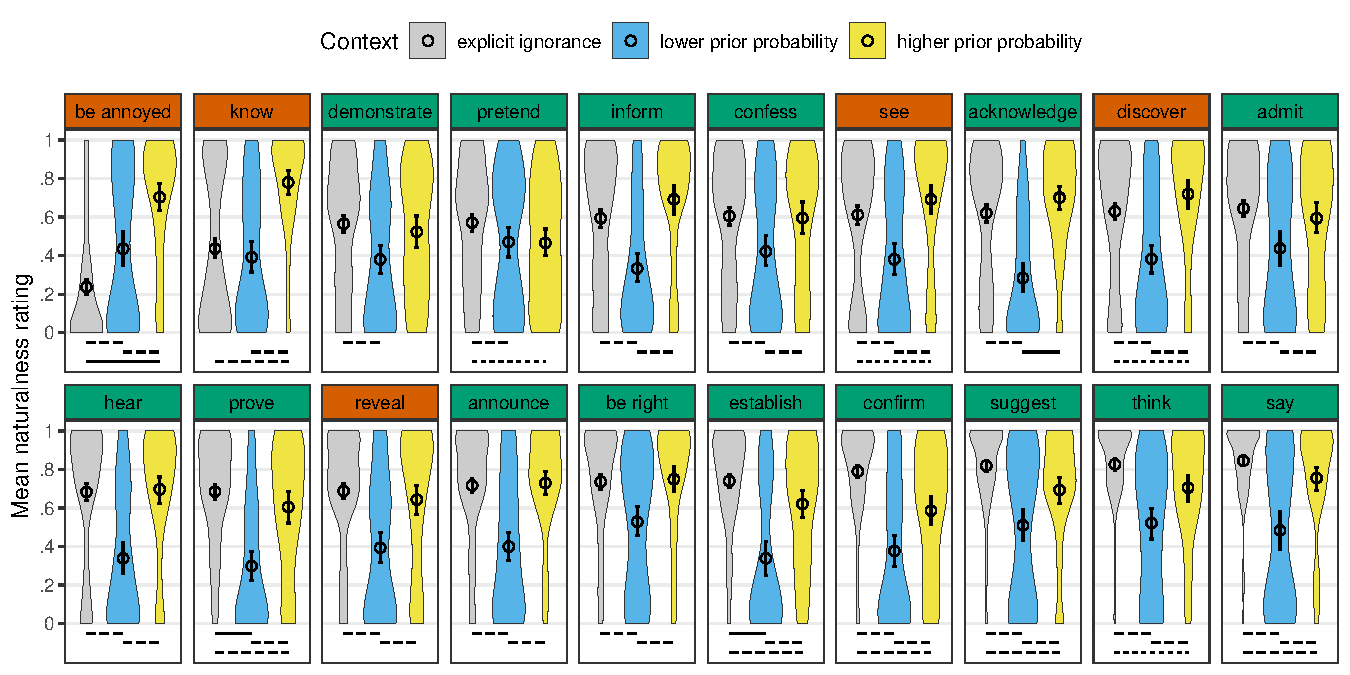
\includegraphics[width=\textwidth]{../../results/main/graphs/naturalness-by-context-and-predicate-with-stats}
\caption{Mean naturalness rating by predicate (\fcolorbox{black}{orange}{factive}, \fcolorbox{black}{green}{nonfactive}) and context, with predicates ordered as in Fig.~\ref{fig:acc-by-expression}. Error bars indicate 95\% bootstrapped CIs. Violin plots indicate kernel probability density of participants' ratings. Below each facet, a line spanning two contexts  indicates that the ratings differ according to the pairwise comparison of contexts. The linetype indicates  whether the difference is at least 1.5 (solid line: ---), below 1.5 but at least 0.5 (dashed line: -- --), or below 0.5 but above 0 (dotted line: \raisebox{1mm}{\ldots}). }\label{fig:acc-by-context}
\end{figure}



% As shown in Table \ref{t:pairwise2},\footnote{The full model output is available here: \url{LINK TO TABLE IN REPO}.{\bf ADD AFTER FINALIZING SCRIPTS}} the model confirms that the effect of context is not uniform for the five factive predicates: The difference between the naturalness ratings in the higher prior probability context and the explicit ignorance context is larger for {\em be annoyed} than for {\em know}, which in turn is larger than for {\em see} and {\em discover}. For {\em reveal} there is no difference, just like for many nonfactive predicates, such as {\em admit, hear, announce} and {\em be right}. The comparison of the lower prior probability context and the explicit ignorance context reveals a positive difference for {\em be annoyed}, no difference for {\em know} and a negative difference for {\em see, discover}, and {\em reveal}. Finally, there is a positive difference between the higher and lower prior probability context for all 20 predicates except for {\em demonstrate} and {\em pretend}.
% 
%\begin{table}[!h]
%\addtolength{\tabcolsep}{-.19em}
%\centering
%\begin{tabular}{r  cccccccccccccccccccc}
%& \rots{\color{orange}be annoyed\color{black}} & \rots{\color{orange}know\color{black}} & \rots{\color{green}demonstrate\color{black}} & \rots{\color{green}pretend\color{black}} & \rots{\color{green}inform\color{black}} & \rots{\color{green}confess\color{black}} & \rots{\color{orange}see\color{black}} & \rots{\color{green}acknowledge\color{black}} & \rots{\color{orange}discover\color{black}} & \rots{\color{green}admit\color{black}} & \rots{\color{green}hear\color{black}} & \rots{\color{green}prove\color{black}} & \rots{\color{orange}reveal\color{black}} & \rots{\color{green}announce\color{black}} & \rots{\color{green}be right\color{black}} & \rots{\color{green}establish\color{black}} & \rots{\color{green}confirm\color{black}} & \rots{\color{green}suggest\color{black}} & \rots{\color{green}think\color{black}} & \rots{\color{green}say\color{black}} \\
%\hline
% higher prior - EIC & \cellcolor{yellow1} & \cellcolor{yellow2} & \cellcolor{white} & \cellcolor{purple3} & \cellcolor{white} & \cellcolor{white} & \cellcolor{yellow3} & \cellcolor{white} & \cellcolor{yellow3} & \cellcolor{white} & \cellcolor{white} & \cellcolor{purple2} & \cellcolor{white} & \cellcolor{white} & \cellcolor{white} & \cellcolor{purple2} & \cellcolor{purple2} & \cellcolor{purple2} & \cellcolor{purple3} & \cellcolor{purple2} \\ 
  lower prior - EIC & \cellcolor{yellow2} & \cellcolor{white} & \cellcolor{purple2} & \cellcolor{purple2} & \cellcolor{purple2} & \cellcolor{purple2} & \cellcolor{purple2} & \cellcolor{purple2} & \cellcolor{purple2} & \cellcolor{purple2} & \cellcolor{purple2} & \cellcolor{purple1} & \cellcolor{purple2} & \cellcolor{purple2} & \cellcolor{purple2} & \cellcolor{purple1} & \cellcolor{purple2} & \cellcolor{purple2} & \cellcolor{purple2} & \cellcolor{purple2} \\ 
  higher - lower prior & \cellcolor{yellow2} & \cellcolor{yellow2} & \cellcolor{white} & \cellcolor{white} & \cellcolor{yellow2} & \cellcolor{yellow2} & \cellcolor{yellow2} & \cellcolor{yellow1} & \cellcolor{yellow2} & \cellcolor{yellow2} & \cellcolor{yellow2} & \cellcolor{yellow2} & \cellcolor{yellow2} & \cellcolor{yellow2} & \cellcolor{yellow2} & \cellcolor{yellow2} & \cellcolor{yellow2} & \cellcolor{yellow2} & \cellcolor{yellow2} & \cellcolor{yellow2} \\ 
  

%\hline
%\end{tabular}
%\caption{Posterior distribution of estimated marginal means of pairwise differences between the three contexts for each expression, with expressions ordered by mean naturalness rating in explicit ignorance context. `EIC' stands for explicit ignorance context. Color coding indicates whether the difference was positive or negative, and the size of the difference; a white cell means that there was no difference: \\
%Positive difference: \colorbox{yellow1}{\makebox[4em][c]{$>=-1.5$}}, \colorbox{yellow2}{\makebox[4em][c]{($-1.5, -0.5]$}}, \colorbox{yellow3}{\makebox[4em][c]{($-0.5, 0]$}} \\
%Negative difference: \colorbox{purple1}{\makebox[4em][c]{$>=1.5$}}, \colorbox{purple2}{\makebox[4em][c]{($1.5,0.5]$}}, 
%\colorbox{purple3}{\makebox[4em][c]{($0.5, 0]$}} 
%}\label{t:pairwise2}
%\end{table}

\paragraph{Discussion.} As mentioned above, contemporary presupposition analyses (e.g., \citealt{heim83,vds92}) assume that presuppositions are by default globally accommodated when they are not entailed by or satisfied in the context, and they can be locally accommodated (e.g., under the polar question operator) to avoid contradiction, uninformativity or problems with binding. Such analyses led us to expect that presuppositions are rated as natural in higher and lower prior probability contexts, as these contexts do not contradict the CCs, make the CCs uninformative, or lead to problems with binding. Contrary to this expectation, the CCs of the five purportedly factive predicates received lower ratings in the lower prior probability context than in the higher prior probability context.\footnote{In the higher prior probability context, our five purportedly factive predicates received ratings roughly comparable to the ratings of the factive predicates investigated in \citealt{mandelkern-etal2020} in their support context. Specifically, in our higher prior probability context, the mean naturalness ratings for the CCs of the five factive predicates ranged from .64 ({\em reveal}) to .78 ({\em know}) on a scale from 0 to 1. In \citepos{mandelkern-etal2020} support context, the CCs of {\em be aware} and {\em be happy} received mean naturalness ratings of about 4.4 and 4.7 out of 7 (based on Fig.~8 in their Appendix).} This result suggests that naturalness ratings are sensitive to the prior probability of content, such that an interrogative with a clause-embedding predicate is judged as more natural in a context in which the CC has a higher prior probability than in a context in which it has a lower prior probability. 

This result has several methodological and theoretical implications. First, this result aligns with the result of \citealt{degen-tonhauser-openmind} based on an inference rating measure, suggesting that inference rating and naturalness rating measures are sensitive to some of the same factors. Second, naturalness ratings in explicit ignorance and support contexts are sensitive to a whole slew of factors, including the (implicit) prosody of the utterance and the defeasibility, at-issueness, and the prior probability of content. The assumption that naturalness ratings in such contexts distinguish presuppositions from nonpresuppositions cannot be maintained.
Finally, for analyses of presuppositions that assume a mechanism of local accommodation, the result means that local accommodation is sensitive to the prior probability of content, not just to whether the content is contradictory or uninformative in the context. 

%One thing that is striking about the naturalness ratings is that for many  predicates the ratings are quite high in both the explicit ignorance and the higher prior probability context (e.g., {\em inform, see, discover, hear, reveal, be right, think, say}). This suggests that interrogatives with these predicates are natural both in contexts in which the speaker is uncertain about the truth of the CC and in contexts in which the speaker believes the CC to have a high probability. This result, which crosscuts the factive/nonfactive distinction, highlights the flexibility with which these predicates are used in discourse, 

  
\section{General discussion}\label{s3}

The experiment was designed to investigate \citepos{mandelkern-etal2020} claim that the measure used in their Exp.~3 provides support for categorical  projection and a categorical distinction between presuppositions and nonpresuppositions. Neither the comparison of naturalness ratings in explicit ignorance contexts  in \S\ref{s:analysis1} nor the comparison of naturalness ratings in explicit ignorance and support contexts in \S\ref{s:analysis2} provided support for this claim. Rather, the results align with that of \citealt{degen-tonhauser-language}, namely that factive predicates are not a natural class that is categorically different from nonfactive predicates. In this section, we discuss theoretical implications of the results.

\subsection{What are presuppositions?}\label{s31}

Contemporary literature like \citealt{mandelkern-etal2020} still frequently treats presuppositions as if they were a homogenous class, by characterizing them as backgrounded content that typically projects out of entailment-canceling environments or by analyzing them as conventionally-coded felicity requirements. However, research on projective content has long recognized that the set of contents that have been called presuppositions is heterogeneous along several dimensions. One dimension of variation that was already mentioned in \S\ref{s1} is projection. Experimental investigations suggest that contents traditionally called presuppositions exhibit variation in the strength of the inference to the content (e.g., \citealt{xue-onea11} on German, \citealt{tonhauser-guarani-variability} on Paraguayan Guaran\'i, and \citealt{demarneffe-etal-sub23,tbd-variability,degen-tonhauser-language} on English). In English, for instance, the CC of {\em discover} is less projective than the CC of {\em know}. These results challenge the traditional characterization of presuppositions as contents that ``typically project''.

A second dimension of variation is whether the content is associated with what \citealt*{brst-lang11} referred to as a `strong contextual felicity' constraint. Some presumed presuppositions are not associated with such a constraint, which means that they are judged to be acceptable in a context that is neutral with respect to the content. This is the case for the CC of {\em know}, illustrated in (\ref{scf}a), which is informative in such a context. Other presumed presuppositions are associated with such a constraint, that is, they are judged to be unacceptable in a context that does not entail or satisfy the content. This is the case for the existence requirement of {\em too}, illustrated in (\ref{scf}b).

\begin{exe}
\ex\label{scf} \citealt[78, 80]{brst-lang11}
\begin{xlist}
\ex A girl backs out of a driveway and hits Susi's car. A woman comes running out of the house, apologizes that her daughter hit Susi's car, and says: \\ She knows that she has to use her glasses to drive.

\ex Malena is eating her lunch, a hamburger, on the bus going into town. A woman who she doesn't know sits down next to her and says:
\\ \infelic Our bus driver is eating empanadas, too.

\end{xlist}
\end{exe}
This variation suggests that analyses of presuppositions as conventionally-coded felicity requirements (e.g., \citealt{heim83,vds92}) generalize an analysis that is empirically justified for contents associated with a strong contextual felicity constraint to contents that can be informative. 

A third dimension of variation is at-issueness, that is, whether the content can address the question under discussion. For instance, as shown in \citealt{tbd-variability}, the pre-state content of {\em stop} and the CC of {\em discover} are more at-issue than the CCs of {\em know} and {\em be annoyed}. This variability challenges a unified characterization of presuppositions as backgrounded content. Finally, there is the dimension investigated in our experiment, referred to as defeasibility in \citealt{simons01} and \citealt{abusch10}. The results of our experiment suggest that contents traditionally called presuppositions exhibit variation in how natural (or: defeasible) they are in explicit ignorance contexts. For instance,  the pre-state content of {\em continue} was rated as less natural than the pre-state content of {\em stop}, which was rated as less natural than the existential content of the {\em it-}cleft, which was rated as less natural than the CC of {\em see}, which was rated as less natural than the CC of {\em reveal}. No unified characterization of `presupposition' is forthcoming from this measure either.

These dimensions of variation strongly suggest that the set of contents traditionally referred to as presuppositions does not constitute a natural class. It is in response to such variation that researchers have developed analyses of subsets of these contents that capture projection variability and do not rely on a conventional specification of felicity conditions (e.g., \citealt{abrusan2011,abrusan2013,abrusan2016,abusch02,abusch10,romoli2015}). A fruitful path forward for contemporary research on projective content is to engage with this variation rather than to keep taking for granted a characterization of `presupposition'  based on projection or an analysis as conventionally-specified felicity conditions.

\subsection{Are there factive predicates?}

As discussed in \citealt{degen-tonhauser-language}, factive predicates are variably defined as predicates whose CC is presupposed (e.g., \citealt{kiparsky-kiparsky70}) or as predicates whose CC is presupposed and entailed (e.g., \citealt{gazdar79a,schlenker10,abrusan2011}). \citealt{degen-tonhauser-language} did not find empirical support for a natural class of factive predicates that is categorically distinct from nonfactive ones: First, based on the results of two experiments designed to investigate the projection of the CCs of (non)factive predicates as well as the analyses of three existing projection datasets with up to 517 (non)factive predicates,\footnote{These datasets were the CommitmentBank (\citealt{demarneffe-etal-sub23}), the VerbVeridicality dataset (\citealt{ross-pavlick2019}), and the MegaVeridicality dataset (\citealt{white-rawlins-nels2018}).} this work suggested that projection does not categorically distinguish factive and nonfactive predicates. Second, based on four experiments designed to investigate the entailment of the CCs of (non)factive predicates as well as analyses of entailment in two of the aforementioned datasets, this work suggested that considering entailment in addition to projection also does not provide support for a natural class of factive predicates that is categorically distinct from nonfactive ones. 

The results presented in \citealt{degen-tonhauser-language} were based on a variety of inference rating measures: In some measures, participants read constructed examples, in others naturally occurring ones; in some, examples were presented with a context, in others without a context; in some, the examples had diverse lexical content, in others, they had minimal lexical content. Across the measures, the clause-embedding predicates were embedded under different entailment-canceling operators, participants were asked to respond to different questions, and participants gave their response on different scales and sliders. Despite this variation, the results invariably suggested that factive predicates are not categorically distinct from nonfactive ones. 

The experiment presented in this paper presents supports \citepos{degen-tonhauser-language} result based on a different measure, namely naturalness ratings in explicit ignorance contexts. The CCs of the five purportedly factive predicates exhibited variation in how natural they were rated when the speaker was explicitly ignorant of the CC, and there were no differences between the CCs of {\em see, discover} and {\em reveal} and several nonfactive predicates. Thus, neither data based on inference rating measures nor data based on naturalness ratings in explicit ignorance contexts provide support for a natural class of factive predicates. As discussed in \citealt{degen-tonhauser-language}, ``the search for a class of factive predicates might continue'' (p.586), but we believe that it is more fruitful to investigate the more fine-grained distinctions between clause-embedding predicates that can lead to a better understanding of their uses in discourse and, hence, the projection of their CCs.

\subsection{Towards a formal analysis of gradient projection}

As mentioned in \S\ref{s1}, \citealt{tbd-variability} observed that the CCs of factive predicates vary in how projective they are,  based on data collected with an inference rating measure. This observation led them to propose that projection is gradient rather than categorical. This proposal was further supported by the results of the experiments and analyses of existing datasets in \citealt{degen-tonhauser-language}, who found that the projection means of the CCs of factive and nonfactive predicates form a gradient rather than being categorically distinct (see Fig.~\ref{fig:dt1a}). \citealt{mandelkern-etal2020}, on the other hand, maintained that projection is categorical and  they claimed that  their naturalness rating measure categorically distinguishes presuppositions and nonpresuppositions.  As discussed above, neither the results presented in \citealt{mandelkern-etal2020} nor the results of our experiment empirically support the claim that projection is categorical. Instead, the results of our experiment provide further empirical support for the proposal that contents associated with different expressions (e.g., the CCs of {\em know, discover} and {\em confess}) do not either project or not project, but rather exhibit quite fine-grained variation in how projective they are.

There are already some suggestions in the contemporary literature on projection for how to deal with projection variation. The analyses of \citealt{heim83} and \citealt{vds92}, which assume that expressions are either presupposition triggers or not, rely on local accommodation to account for examples in which presuppositions do not project (for discussion see, e.g., \citealt{djaerv-bacovcin2020,mandelkern-etal2020}). However, as discussed in detail in \citealt{tbd-variability}, it is not clear that local accommodation can capture the observed by-content variation in a principled way, as such analyses would need to assume, for instance, that the CC of {\em discover} is more amenable to local accommodation than the CC of {\em know}. Another challenge for these analyses is the observation that the CCs of nonfactive predicates are also projective,  sometimes even more so than the CCs of factive predicates. Because nonfactive predicates do not trigger a presupposition in analyses like \citealt{heim83} and \citealt{vds92}, these analyses make no predictions about the projection of the CCs of nonfactive predicates (see \citealt{degen-tonhauser-language} for further discussion).

Another set of projection analyses was developed to capture the projection of content associated with soft triggers (e.g., \citealt{abusch02,abusch10, abrusan2011,abrusan2016,romoli2015,simons-etal2017}). These analyses (which differ in detail)  were developed to capture that the projection of content associated with soft triggers is more easily suspended than that of hard triggers. Given such analyses, a three-way distinction in projection can be predicted: Content that is conventionally marked as a presupposition (like the prejacent of {\em too} and {\em also}) is expected to be more projective than the content of soft triggers (like the prejacent of {\em stop} or the CC of {\em discover}), which in turn is expected to be more projective than content contributed by expressions that have traditionally not been analyzed as presuppositions (like the CC of {\em confess}). While this is a promising step in the right direction, it obviously falls short of fully capturing the observed projection variability, for instance, that the CC of {\em know} is more projective than that of {\em discover}, which in turn is more projective than that of {\em reveal}, or that contents associated with nontriggers, such as the CCs of nonfactive predicates, may be projective, too, albeit to varying degrees (see \citealt{tbd-variability} and \citealt{degen-tonhauser-language} for discussion). 

This situation suggests that a promising avenue for future research is to continue investigating distinctions between expressions associated with projection inferences (see \S\ref{s31}).  Understanding the dimensions along which projection inferences do or don't differ will lead to a refined taxonomy of such inferences (for a preliminary taxonomy see \citealt{brst-lang11}). The differences between empirically-motivated classes of projection inferences can, in turn, be decisive in identifying inferences already captured by extant analyses and inferences for which novel analyses must be developed.


%Where does this leave us with the question of whether the projection of content is categorical or gradient? The challenge is clear: Proponents of either position must confront the observed by-content projection variability and develop analyses that capture the variability in a principled way. As none of the contemporary projection analyses are able to do so, one might say that the verdict is still out. The empirical evidence, however, seems to favor the hypothesis that projection is gradient, as there is, to date, no empirical evidence that projection is categorical, and empirical evidence from several different measures that it is gradient.

%\footnote{Another potential source of projection variability is speaker belief. \citealt[498f.]{tbd-variability} pointed out that speaker belief could be categorical (the speaker either believe that the content is true or they are uncertain) or gradient (the speaker believes that the content is true to some degree). On either view, interpreters might draw projection inferences of different strengths due to uncertainty about (the degree of) the speaker's belief.}  

%What the question is not about is the projection of {\em utterance content}. What we mean by that is the strength of the projection inference that a particular interpreter draws from a particular utterance of a sentence in which a content is contributed in the scope of an entailment-canceling operator. The empirical evidence pointed to in \S\ref{s1} shows that different interpreters draw projection inferences of varying strength. For instance, as shown in Fig.~\ref{fig:dt1a-JULIAN}, the participants of \citepos{degen-tonhauser-language} Exp.~1a drew projection inferences of varying strength for the CC that Julian dances salsa from utterances of the interrogative {\em Did Scott discover that Julian dances salsa?} It is uncontroversial that this utterance content variability is gradient, not categorical. It is gradient because the projection of utterance content is sensitive to several factors on which interpreters differ, including their prior beliefs about the speaker or about the utterance content, their perception and interpretation of the prosodic realization of the utterances, and their assumptions about the question under discussion addressed by the utterance (e.g., \citealt{djaerv-bacovcin2020,degen-tonhauser-openmind,mahler2020,mahler-thesis,tonhauser-salt26,tbd-variability,tonhauser-etal-sub23}).
%
%\begin{figure}[h!]
%\centering
%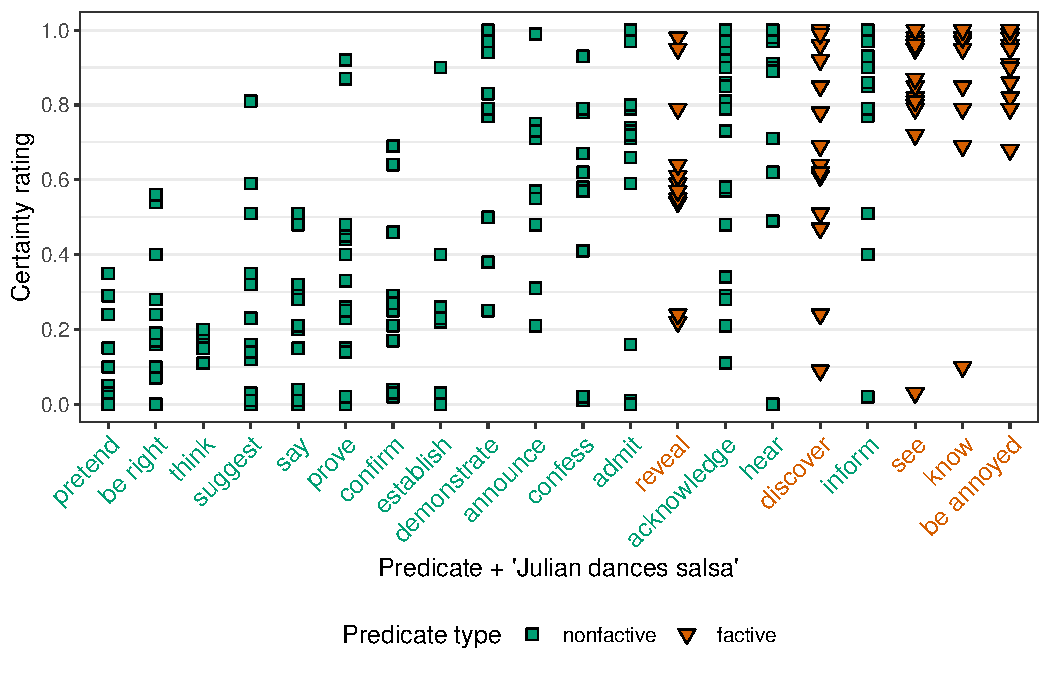
\includegraphics[width=.8\textwidth]{../../results/main/graphs/mean-certainty-by-predicateType-JULIAN}
%\caption{Participants' certainty ratings (measuring projection) of the CC that Julian dances salsa for the 20 \color{orange}factive \color{black} and \color{green}nonfactive \color{black} predicates investigated in Exp.~1a of \citealt{degen-tonhauser-language}.}\label{fig:dt1a-JULIAN}
%\end{figure}

\section{Conclusions}\label{s4}

For many decades the term `presupposition' has served researchers well to refer to content with properties distinct from, for instance, entailments, conventional implicatures and conversational implicatures. However, over the past two decades, both empirical and theoretical research has pointed out that the set of contents typically referred to as presuppositions is not as homogenous as perhaps initially assumed, resulting in theoretical analyses of particular subsets and an understanding of multiple dimensions of empirical variation among this set of contents. Against this background, the claim in \citealt{mandelkern-etal2020} that there is an empirical measure that categorically distinguishes presuppositions from nonpresuppositions sparked hope that there might be, after all, a way of preserving the term `presupposition' as a well-defined notion in the way it has been traditionally used.  Unfortunately, the results of our experiment did not support this claim, instead providing further evidence for variation among the set of contents traditionally referred to as presuppositions. We suggest retiring the term `presupposition' or, at least, confining its use to a particular subtype of projective content, such as content associated with a strong contextual felicity constraint.




% end document here for word count
%\end{document}

\bibliographystyle{cslipubs-natbib}
%\bibliographystyle{/Users/tonhauser.1/Library/Latex/cslipubs-natbib}
\bibliography{bibliography}

\newpage

\section*{Supplemental materials}

\appendix

\setcounter{page}{1}
%\renewcommand{\thetable}{A\arabic{table}}

\setcounter{table}{0}
\renewcommand{\thetable}{A\arabic{table}}

\setcounter{figure}{0}
\renewcommand{\thefigure}{A\arabic{figure}}

\section{Experiment stimuli}\label{a:clauses}

The twenty clause-embedding predicates used in the experiment are the same as in \citealt{degen-tonhauser-openmind,degen-tonhauser-language}:

\begin{exe}
\ex\label{predicates}
\begin{xlist}
\ex Factive: be annoyed, discover, know, reveal, see
\ex Non-factive: acknowledge, admit, announce, be right, confess, confirm, establish, hear, inform, pretend, prove, say, suggest, think
\end{xlist}
\end{exe}
Eventive predicates, like {\em discover} and {\em hear}, were realized in the past tense and stative predicates, like {\em know} and {\em be annoyed}, were realized in the present tense. The direct object of {\em inform} was realized by the proper name {\em Sam}. Each clause-embedding predicate was paired with a unique subject proper name. The speaker of the target stimuli was realized by a randomly sampled unique proper name. 

The following list shows the 20 clauses that realized the complements of the predicates in the target stimuli, together with their lower and higher probability facts, respectively, that realized the preceding declarative sentences in the two support contexts.

\begin{enumerate}[leftmargin=4ex,itemsep=-2pt]
\item Mary is pregnant. Facts: Mary is a middle school student / Mary is taking a prenatal yoga class
\item Josie went on vacation to France. Facts:  Josie doesn't have a passport / Josie loves France 
\item Emma studied on Saturday morning. Facts: Emma is in first grade / Emma is in law school 
\item Olivia sleeps until noon. Facts: Olivia has two small children / Olivia works the third shift
\item Sophia got a tattoo. Facts: Sophia is a high end fashion model / Sophia is a hipster
\item Mia drank 2 cocktails last night. Facts: Mia is a nun / Mia is a college student
\item Isabella ate a steak on Sunday. Facts: Isabella is a vegetarian / Isabella is from Argentina
\item Emily bought a car yesterday. Facts: Emily never has any money / Emily has been saving for a year
\item Grace visited her sister. Facts: Grace hates her sister / Grace loves her sister
\item Zoe calculated the tip. Facts: Zoe is 5 years old / Zoe is a math major
\item Danny ate the last cupcake. Facts: Danny is a diabetic / Danny loves cake
\item Frank got a cat. Facts: Frank is allergic to cats / Frank has always wanted a pet
\item Jackson ran 10 miles. Facts: Jackson is obese / Jackson is training for a marathon
\item Jayden rented a car. Facts: Jayden doesn't have a driver's license / Jayden's car is in the shop
\item Tony had a drink last night. Facts: Tony has been sober for 20 years / Tony really likes to party with his friends
\item Josh learned to ride a bike yesterday. Facts: Josh is a 75-year old man / Josh is a 5-year old boy
\item Owen shoveled snow last winter. Facts: Owen lives in New Orleans / Owen lives in Chicago
\item Julian dances salsa. Facts: Julian is German / Julian is Cuban
\item Jon walks to work. Facts: Jon lives 10 miles away from work / Jon lives 2 blocks away from work
\item Charley speaks Spanish. Facts: Charley lives in Korea / Charley lives in Mexico
\end{enumerate}

\section{Filler and practice stimuli}\label{a:fillerPractice}

The following list shows the four filler stimuli where the interrogative was expected to receive high naturalness ratings in the context of the preceding declarative sentence. The values in parentheses indicate the mean naturalness rating that each of the four filler stimuli received. As shown, the third filler stimulus did not receive the expected high naturalness mean ratings, probably because participants were unwilling to accommodate that Hendrick has a car in a context in which Hendrick was looking to buy a car. This filler stimulus was therefore not used to exclude participants' data. 

\begin{enumerate}[leftmargin=4ex,itemsep=-2pt]

\item I don't know if Samantha has a new hat. Does Samantha have a new hat? (.89)

\item  I don't know if this pizza has mushrooms on it. Does this pizza have mushrooms on it? (.87)

\item Hendrick was looking to buy a car. Was Hendrick's car expensive? (.5)

\item Mary visited her aunt yesterday. Is Mary's aunt sick? (.91)

\end{enumerate}

\noindent
The following list shows the four practice stimuli in the order in which they were presented to the participants. Participants were able to advance to the experiment only if they gave a naturalness rating higher than .6 for the first and third stimulus, and a naturalness rating lower than .4 for the second and fourth stimulus.

\begin{enumerate}[leftmargin=4ex,itemsep=-2pt]

\item I have no idea where Natalie is from. Is Natalie from the USA?

\item I don't have any sisters. Have you met my sister yet?

\item I am going on vacation to Ireland. Does Fritz realize that Joe is going with me?

\item I have no idea if Anna has any dogs. Is Samuel glad that Anna fed her dogs?

\end{enumerate}

%\section{Model output: Pairwise comparison of expressions}\label{a:analysis1}
%
%{\bf JT PROPOSES TO LEAVE OUT THIS AND THE NEXT FIGURE}
%
%Fig.~\ref{fig:comparisons1} provides a graphical representation of the results of the pairwise comparisons between the ratings for each expression in the explicit ignorance context. The full model output in table form is available here: \url{LINK TO TABLE IN REPO}.
%
%\begin{sidewaysfigure}[h!]
%\centering
%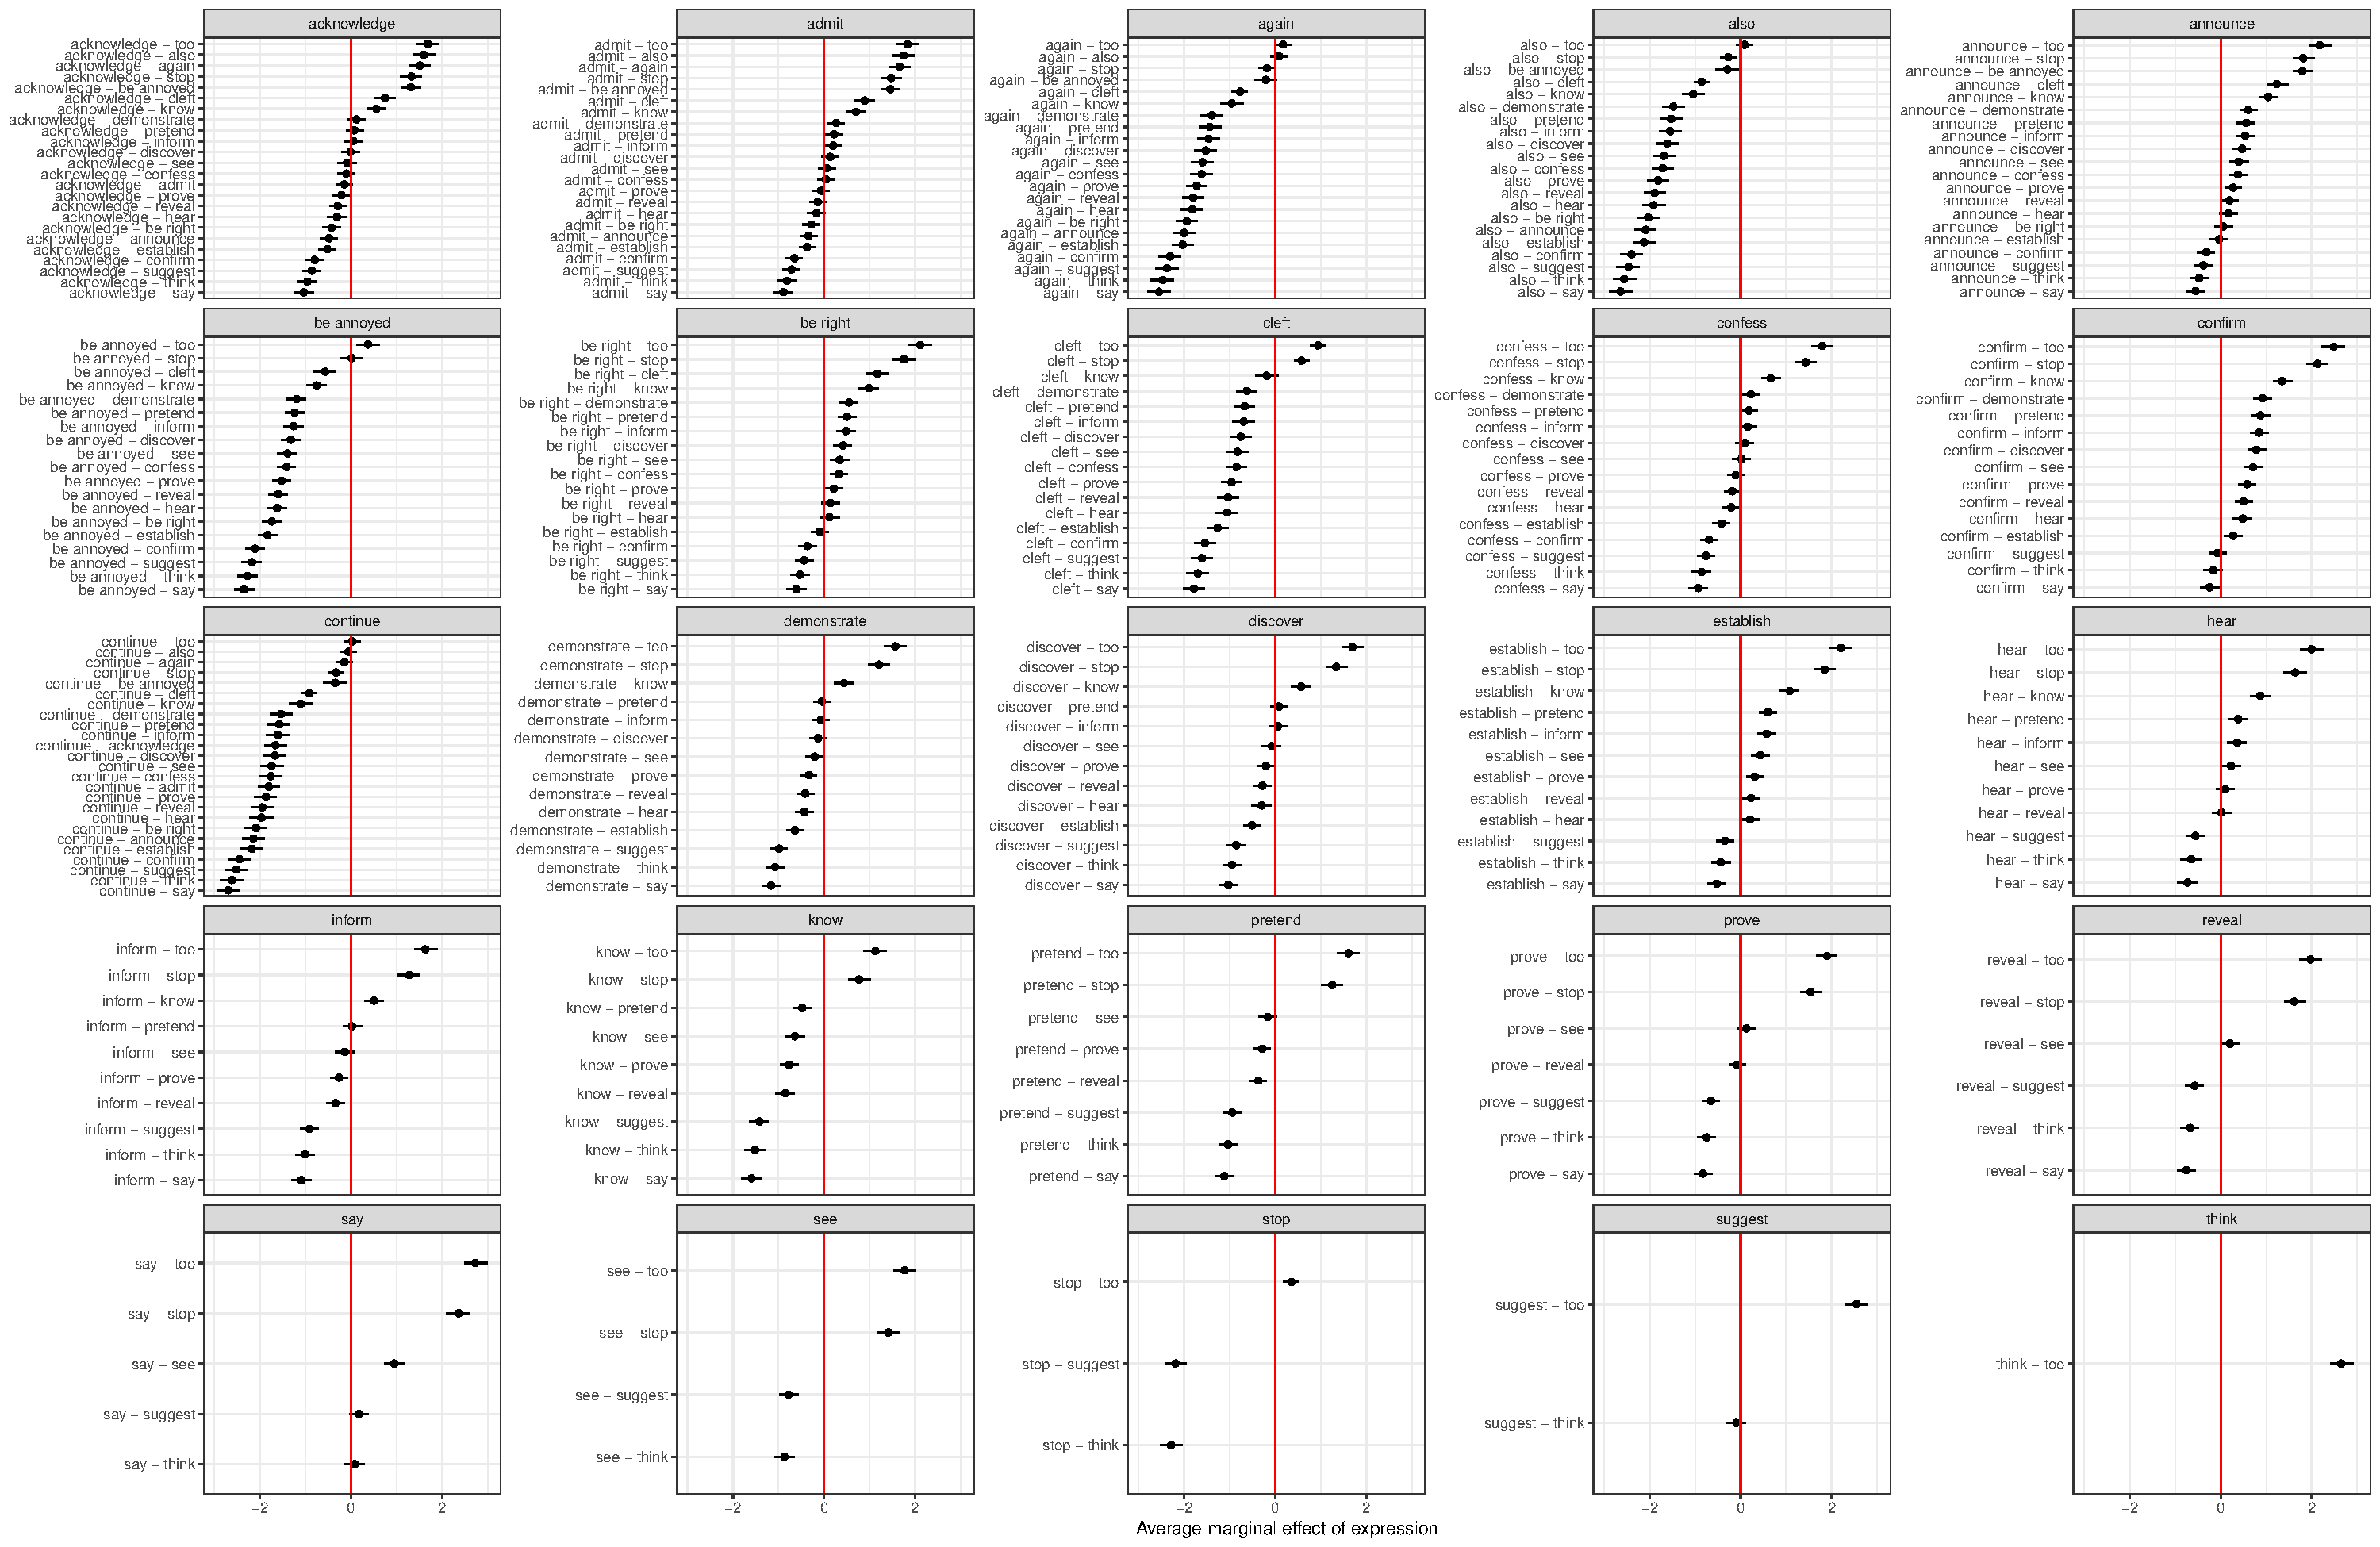
\includegraphics[width=\textwidth]{../../results/main/13explicitIgnorance/graphs/comparisons-in-EIC}
%\caption{.}\label{fig:comparisons1}
%\end{sidewaysfigure}
%
%\section{Model output: Pairwise comparison of contexts}\label{a:analysis2}
%
%Fig.~\ref{fig:comparisons2} provides a graphical representation of the results of the pairwise comparisons of the ratings in the three contexts for each of the 20 predicates. The full model output in table form is available here: \url{LINK TO TABLE IN REPO}.
%
%\begin{figure}[h!]
%\centering
%\includegraphics[width=.8\textwidth]{../../results/main/13explicitIgnorance/graphs/context-comparisons}
%\caption{.}\label{fig:comparisons2}
%\end{figure}
 
\end{document}

